% \begin{savequote}[8cm]
% Alles Gescheite ist schon gedacht worden.\\
% Man muss nur versuchen, es noch einmal zu denken.

% All intelligent thoughts have already been thought;\\
% what is necessary is only to try to think them again.
%   \qauthor{--- Johann Wolfgang von Goethe \cite{von_goethe_wilhelm_1829}}
% \end{savequote}

\chapter{\label{ch:xai}Using Post-Hoc Explainable AI to Identify Talent: Explaining an Applicant Scoring Algorithm with Shapley Values}

% Notes
% Can we replicate misleading explanations? We have data from this year and last.
% Are there classes of cases which are plausibly connected to the types of areas that the old non-SHAP decision-making process would have yielded? Can we independently identify these in the new cohort?
% Maybe: does the new “SHAP” process reduce surprise/disagreement with the algorithm
% Can we do something qualitatively?
% How does SHAP have the right kind of effect on decision-making
% Could we measure the magnitude of disagreement between humans and algorithms?
% Then qualitatively, ask people why they disagreed with algorithm scores?
% It’s hard to tie this stuff specifically to the under/over-reliance stuff unless we can argue that more disagreement is good
% We don’t have ground truth, so the misleading stuff is difficult, but we can argue that disagreement/engagement are both good. We can qualitatively compare the richness/level of understanding/ perceived helpfulness.
% Do they have more reasons for disagreeing? More specific reasons?
% Fundamental thought: if SHAP helps the decision makers understand the reason why, but we don’t care about that factor, wouldn’t it be better to change the model so as to not consider that factor as much? Maybe explanation tools are a way of modifying the model here? Can the case study / utility be a change to the model? Maybe decision-makers need to be in the middle of their decision-making process to reconsider the principles, and maybe these decisions are best made using SHAP?
% Alternative case study idea: maybe various reviewers meet and extract generalisations from the SHAP charts they’ve been using?
% The idea of individual justice: no set of criteria exists that correctly applies to every case; under this principle, the value of SHAP is to say that “this particular case is an exception to the model, since you don’t want to mess with it in general, you just want to make an exception in this case”
% The underlying model is trying to predict accept/reject based on previous candidates, which is sort of a ground truth, but not the only truth that decision-makers are interested in; this is a major difference from the misleading explanations thing
% Another major difference: decision-makers have access to a lot of information the model doesn’t; part of the role of SHAP is to tell decision-makers when that info is important
% It sounds like the evaluation is qualitative / not-based-on-ground-truth. It’s instead based on decision-maker feedback about when they rely on the explainer system
% More satisfying to have some case study
% Can I collect with/without SHAP information on how they collect decisions?
% Could we apply SHAP to previously made decisions and use SHAP to elucidate the past year confusions? This was a part of the design process
% Does this necessarily need to be qualitative?
% Also: do we want to change the model next year based on the decisions made with this algorithm? I.e., should we rely more or less on specific features? This is sort of necessarily qualitative. Also, this could be taken from the design process, since this happened in the interviews
% This makes a good argument for why we can’t just do an RCT 

\minitoc

\section{Introduction}
Post-hoc explainable AI (xAI) systems have been oft maligned as poor tools for decision support. \textcite{Lipton} cautions that well-intentioned explanation design may yield ``misleading but plausible'' explanations, and \textcite{Miller_2023} notes that these post-hoc xAI methods provide justification for the underlying AI models and their outputs rather than allowing users to make their own informed decisions \cite{Miller_2023}. This has, in recent years led to a shift away from post-hoc xAI entirely \cite{Lipton,Miller_2023,kumar_problems_2020,Bastounis_Campodonico_vanderSchaar_Adcock_Hansen_2024}. The core of both critiques is that explanations may induce misplaced explainee trust in model outputs. Indeed, there is evidence that such xAI systems do induce trust in the underlying model \cite{Lai-and-Tan,Jacobs-et-al}. In response, research using xAI as a decision support tool (DST) often eschews post-hoc, model-agnostic explanations in favour of new paradigms such as \textcite{Miller_2023}'s evaluative AI for decision-makers and \textcite{Karimi_Schölkopf_Valera_2021}'s causal models for decision subjects.

But have we been too hasty in rejecting these older methods? Underlying this shift away from xAI is the assumption that approaches will be deployed to increase trust in particular outputs in decision support contexts, even though such trust may be unwarranted when outputs are wrong. But is this always the case? Might these trust-inducing xAI be usefully deployed elsewhere, such as for post-decision evaluation of models and decision making processes?

We introduce a \emph{decision stage} distinction to help consider the benefits and risks of post-hoc interpretability tools as DSTs. We distinguish between: the \emph{in-process} stage, where AI outputs and post-hoc explanations are used to support human decision-makers in confirming or overriding the `primary' decision the model output advises on, and the \emph{ex-post} stage, where the primary decision has already been made, and the xAI is offered to inform second-order decisions about the decision-making process. (E.g., between application cycles, recruitment and selection practitioners examine their prior decision-making procedures and seeks to make decisions that improve them for the next cycle \cite{li2020hiring}.) We seek to answer two research questions (RQs):

\begin{enumerate}
    \item[(RQ1)] Do post-hoc explanations, when used as \emph{in-process} DSTs, induce unwarranted trust in the explainee?
    \item[(RQ2)] If post-hoc xAI methods induce unwarranted trust \emph{in-process}, could they still be useful \emph{ex-post}?
\end{enumerate}

At the \emph{in-process} stage, we run an online study to discern whether the problem of unwarranted trust is specific to xAI. We investigate \textcite{Lundberg-and-Lee,Ribeiro-et-al-anchors}'s popular methods, SHapley-based Additive exPlanations (SHAP) \cite{Lundberg-and-Lee} and Scoped Rules (Anchor) \cite{Ribeiro-et-al-anchors}, respectively, to see if they induce unwarranted trust. We also investigate a `Confidence' explanation consisting of the model's confidence statistic to determine if the problem of unwarranted trust is unique to explanations per se, or applies more generally to the presentation of any information that could increase positive perceptions of the AI's performance. We ask participants to \emph{estimate a person's salary} \cite{Kohavi} or \emph{predict whether someone will be severely delinquent in making a credit payment} \cite{GiveMeSomeCredit} with the help of an AI output and with or without an explanation. We find that SHAP explanations do increase unwarranted trust in AI outputs, but that Confidence does as well. We find no such effect for Anchor. This suggests the problem of unwarranted trust is not unique to xAI per se, and is rather a symptom of generic post-hoc justifications.

Having identified a core problem with some kinds of \emph{in-process} xAI, we consider whether they have any potentially redeeming features if deployed at the \emph{ex-post} level through a series of participatory design workshops. We refine our attention to SHAP because critiques by \textcite{Lipton} and \textcite{Miller_2023} apply most squarely to it. We contend that, in an \emph{ex-post} context, this induction of unwarranted trust is less problematic, as primary decisions have already been made and thus trust in the AI outputs is not at issue. We ask participants to \emph{refine a scholarship selection algorithm} with the help of SHAP-based explanations. Through these workshops we find that, while SHAP explanations may induce unwarranted trust in specific model outputs, they can still be useful to drive process change in organisations.

Our primary contributions in this piece are:

\begin{enumerate}
    \item Quantitative findings indicating that the problem of explanation-induced unwarranted trust extends to generic post-hoc justifications, but that such criticism only applies \emph{in-process}.
    \item Qualitative findings that post-hoc explanations, properly presented, can make useful \emph{ex-post} DSTs.
\end{enumerate}

\section{Background}
\subsection{A Brief History of Explainable AI}\label{ssec:history}
\textcite{Ribeiro-et-al-lime}'s Local Interpretable Model-agnostic Explanations (LIME), which identifies important features (creating a `feature-based' explanation) grew popular as an offering for explanations of Computer Vision (CV) models. \textcite{Ribeiro-et-al-lime} demonstrated the explanation method on a task classifying huskies and wolves. By highlighting that the model used snow to recognise huskies, LIME would help a user spot what portions of an image were likely to be causing the model's classifications. By highlighting that the model used snow to recognise huskies, rather than e.g. their coat pattern, the user might come to understand the model's abilities and limitations, and calibrate their trust accordingly.

The explanation paradigm established by LIME was shortly thereafter applied to non-CV tasks. Tasks based on tabular data, in particular, were often explained using LIME \cite{Zerilli}. Subsequent xAI methods have revised the feature-centric paradigm established by LIME to better fit this new data type. \textcite{Lundberg-and-Lee}'s SHAP offers another way of calculating the influence of each feature wherein the sum of the influences of each feature (plus a `bias' term) equals the model's output, and has since grown ubiquitous in the xAI field \cite{Weerts-et-al-evaluation}.

But while the feature-based methodology underlying LIME and SHAP is useful for identifying error in the computer vision case, this relies on the human evaluator comparing explanation outputs to their (at least partial) knowledge of the ground truth (i.e., when the LIME explanation highlights a portion of the image, the human evaluator must rely on their knowledge of the ground truth to identify whether what is highlighted is relevant). While this may make good sense in cases such as the task classifying huskies and wolves, more contentious applications involve less obvious decisions where, even with access to feature space, a human reviewer might not be able to deduce the correct ground truth classification \cite{kumar_problems_2020,Markus-et-al}.\footnote{This is just one of many problems with feature importance explanations. \textcite{Miller} outlines a list of desiderata that model interpretability methods should satisfy; he points to a need for: contrastive, counterfactual, selective, and social explanations; the feature importance statistics yielded by LIME and SHAP are none of these.} But if these explanations are provided in cases where they do not help users identify cases where the AI output is incorrect, they can only serve to increase trust in the outputs, and cannot serve to decrease said trust where it is not warranted; explanations of AI outputs should only be reassuring if they might have not been.

`Example-based' explanations respond to many of these critiques. \textcite{Wachter-et-al}'s Counterfactual Explanations (CE) presents an example counterfactual to the input, showing the user a similar feature value with a different model output. \textcite{Mothilal-et-al}'s DIverse Contrastive Explanations (DICE) operate similarly, presenting multiple intentionally diverse counterfactuals to give the explainee a better sense of the many ways that the feature space could be perturbed. These counterfactuals serve to give explainees a glimpse into local model behaviour – if the model behaves strangely in any of these similar examples, it is likely untrustworthy in the original instance. However, these explanations are not without their own critiques. In particular, counterfactual explanations are subject to a Rashomon effect; i.e., for any explainable point, multiple counterfactuals may be equally valid. \textcite{Miller} argues that xAI methods should be selective in what they show explainees so as to not overwhelm them, but if there are many valid counterfactuals, we must then choose between showing an explainee all counterfactuals and violating selectivity, or selecting only a few counterfactuals and biasing the explanations.

\textcite{Ribeiro-et-al-anchors}'s Anchor retains the contrastive benefits of CE without suffering the same Rashomon paradox. The algorithm yields a set of conditional statements that help bound the model's output in a region surrounding the actual point. Similarly, \textcite{Ustun-et-al}'s Actionable Recourse (Recourse) offers decision subjects rules guiding what they must change in order to receive a different determination. These explanations meet \textcite{Miller}'s selectivity maxim without ad-hoc simplifications.

\subsection{A Taxonomy of Explanation Algorithms}
In much of the xAI literature, descriptors such as ``post-hoc'' or ``model-specific'' are used to describe types of explainability. We provide a taxonomy of them here and in Figure \ref{fig:taxonomy}.

\begin{figure}[htbp]
    \centering
    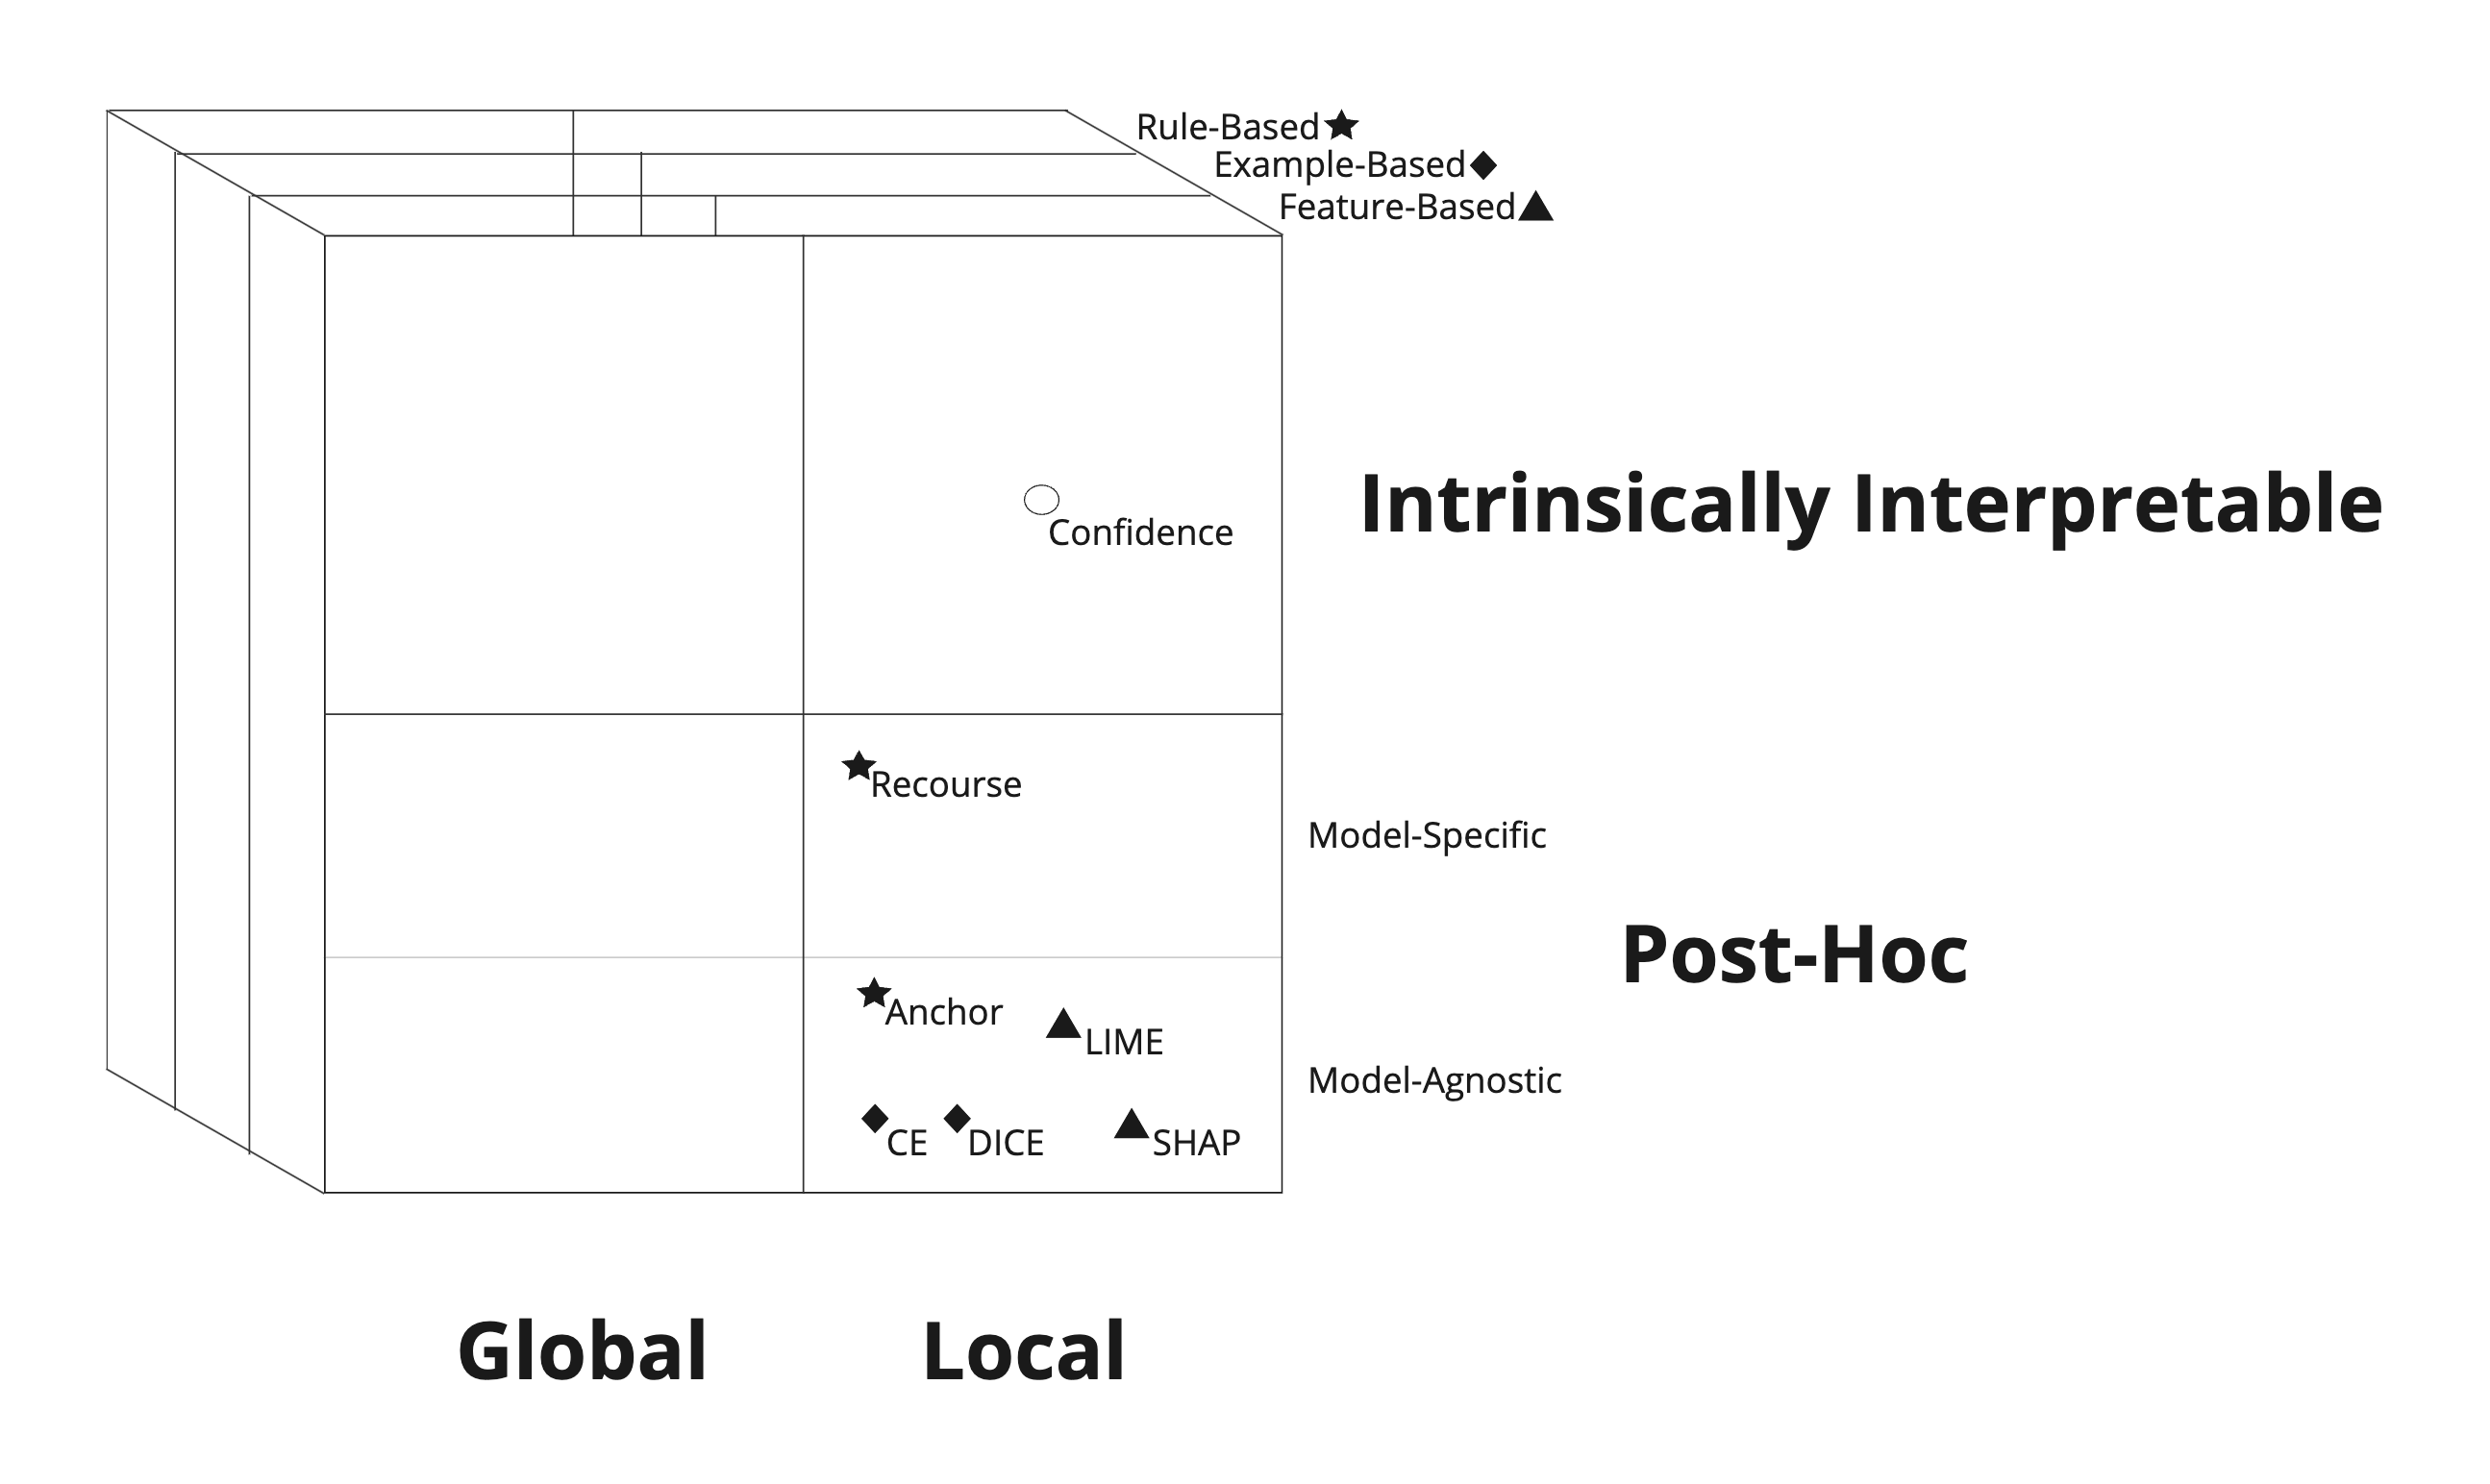
\includegraphics[width=.9\textwidth]{xai/taxonomy.png}
    \caption{Explainable AI methods are separated into types by this taxonomy. We focus primarily on kinds of post-hoc (model-agnostic) explanations, and highlight a number of explanations following different philosophies (SHAP and Anchor are of particular interest, as both recur in our analyses), but we also consider model confidence statistics, which follow none of these philosophies.}
    \label{fig:taxonomy}
\end{figure}

We begin by broadly categorising the space of explainable AI into two subgroups: intrinsically interpretable models and post-hoc explanations \cite{Molnar}. Though intrinsically interpretable models offer solutions for interpretability and often present their own explanations, we (and the xAI critiques we engage with) focus primarily on post-hoc explanations. Key here is that, while intrinsically interpretable models are inherently model-specific, post-hoc methods may reap the benefits of model-agnosticity; thus, a single method may be used on any number of underlying models. This feeds into many of the main criticisms – \textcite{Lipton}'s argument about misleading explanations restricts itself to post-hoc models, we contend, because of this frequent ignorance about the model's internal processes.

Alternatively, explanations can be separated into global methods, which explain entire models, and local methods, which explain individual decisions \cite{Molnar}. Though similar, the distinction between local and global differs from our \emph{decision stage} distinction as the decision stages distinction does not identify the scope of the explanation itself, but rather identifies the scope of the decision. Local explanations, of course, lend themselves best to \emph{in-process} decisions, but one could supply a global explanation here instead. And \emph{ex-post} decisions are varyingly informed best by local or global explanations. We focus on local explanations.

Finally, explainability methods could be instead subdivided by the design philosophy of their outputs \cite{Friedrich-and-Zanker}. Some methods are `Feature-Based' in that they offer feature importance statistics. Other `Example-Based' explanations give examples. Yet other `Rule-Based' explanations offer rules that guide decision-making. Many explanations follow none of these paradigms. Model confidence statistics, for example, do not subscribe to any such design philosophies, but are often used as explanations in place of explainable AI systems \cite{Zhang-et-al}. All explanations we mention, as well as where they fit on this taxonomy, are detailed in Figure \ref{fig:taxonomy}.

\subsection{Ethical Considerations of Employing xAI Systems as DSTs}
Researchers bring up many concerns about using AI systems in general as DSTs. The most relevant bodies of concern for us come from literature around scholarship selection and recruitment. One major concern is that AI algorithms amplify human biases \cite{MikePerkins_JasperRoe_2023}. Though this concern does and should limit applications of certain AI systems, it must be weighed against pre-existing human bias in pipelines. That is, a system might be less biased than what it replaces. Furthermore, a system might even be used to help holistic reviewers identify and mitigate their own biases \cite{Alvero_Arthurs_antonio_Domingue_Gebre-Medhin_Giebel_Stevens_2020}.

More broadly, \textcite{Alvero_Arthurs_antonio_Domingue_Gebre-Medhin_Giebel_Stevens_2020} note that, while AI researchers tend to think of fairness on a population level, recruiters (and, we contend, practitioners in related fields) think of fairness on an individual level. I.e., when making decisions based on qualitative information about a candidate in a process known as holistic review, reviewers are thinking of being fair to the candidate in front of them. But new AI tools blur the quantitative and the qualitative: what was once a simple score can now be a full explanation, and what was once a human-gradable essay could be automatically given a score. There is, we contend, space in these processes for tools that can help reviewers understand the qualitative and quantitative contexts surrounding the decisions they make.

\subsection{Evaluating Unwarranted Trust in a Model}
In order to evaluate whether an explanation induces unwarranted trust, we must evaluate both trust and warrantedness. We begin with trust. \textcite{Jacovi-et-al} define trust in an AI system as characterised by two properties: ``the vulnerability of the user, and the ability to anticipate the impact of the AI model's decisions''; \textcite{Vereschak-et-al} similarly isolate three elements: ``trust is linked to a situation of vulnerability and positive expectations, and is an attitude''; \textcite{Lee-and-See} give a similar definition of trust: ``An attitude that an agent will achieve an individual's goal in a situation characterized by uncertainty and vulnerability''. In all definitions, we see \emph{vulnerability} emerge as a key concept, and we variably also see that trust is characterised by \emph{uncertainty} and \emph{expectations}. Finally, we see that the definitions used with respect to evaluations of AI systems tend to be attitudinal in nature. However, though \textcite{Vereschak-et-al} suggest that trust is an unobservable variable, they term behaviours emergent from trust, rather than the attitude itself, `reliance'. 

The form of trust detailed by \textcite{Vereschak-et-al} is elsewhere called `attitudinal' trust \cite{Crites-et-al}. This form of trust is the one most often considered in human-centred AI, and much of the research discussing explainable AI focuses on this form of trust \cite{Vereschak-et-al, Ford-et-al, Bansal-et-al, Yin-et-al}. However, less frequently documented is a second, `behavioural' form of trust \cite{Crites-et-al}. When \textcite{Jacovi-et-al,Lee-and-See} argue that trust is measurable through such behaviours as reliance, we contend that they are speaking not of attitudinal trust, but rather of behavioural trust. Unlike attitudinal trust, behavioural trust does not rely on the participants' understanding of the term matching academic definitions, or on their estimates of their own trust accurately capturing what we seek to measure \cite{Jacovi-et-al}. This more closely maps onto how explanations impact on the actual decisions made by humans-in-the-loop in practice.

Though attitudinal and behavioural trust are conceptually similar, research is mixed on the existence and strength of correlation between the two constructs \cite{Ahmed-and-Salas, Kim}. As we wish to take a full account of trust in AI systems, we must consider both forms of trust.

We now turn to the warrantedness of said trust. \textcite{Vereschak_Alizadeh_Bailly_Caramiaux_2024} establish a clear distinction between trust and trustworthiness, and observe this distinction in decision-makers and decision subjects alike. That is to say, all parties involved agree that it is at least possible to place unwarranted trust in an algorithm \cite{Vereschak_Alizadeh_Bailly_Caramiaux_2024}. However, when it comes the the question of whether a given model output is trustworthy, opinions are more mixed. Some argue that certain uses of AI systems are inherently untrustworthy, but for many others, the trustworthiness of these systems is merely a matter of their accuracy \cite{Rebitschek_Gigerenzer_Wagner_2021}. \textcite{Rebitschek_Gigerenzer_Wagner_2021} find that, in the aforementioned case of credit estimation, potential decision subjects tend to simply place higher accuracy requirements on their willingness to trust an AI system. \textcite{Jacovi-et-al} similarly conclude that a model's trustworthiness is related to properties such as accuracy, robustness, and bias. However, unlike accuracy, a model may be trustworthy in some contexts, and not in others. I.e., a model may be sufficiently accurate so as to be trustworthy when used to give rough estimates, but insufficiently accurate for use in high-stakes decisions. In the case of specific instances of model outputs, though, the question of trustworthiness is more straightforward: when a system outputs a correct (or an incorrect) result, that result is trustworthy (or untrustworthy).

\subsection{A Taxonomy of Critiques}
There is a large body of studies that empirically evaluate xAI methods. In some cases, an xAI method is evaluated not with human subject experiments but rather with analysis of mathematical properties \cite{Doshi-Velez-and-Kim}. These critiques range from \textcite{kumar_problems_2020}'s argument that SHAP explanations lack desired properties like contrastiveness to \textcite{Lundberg-and-Lee}'s argument that LIME's mathematical properties make it unsuited to tabular data.

However, while these evaluations are instructive in that they provide interesting new perspectives on technologies, they do not help us evaluate whether utilising these explanations as DSTs is problematic in practice. To determine this, we turn to evaluations that involve humans using an AI system to perform some task \cite{Ribeiro-et-al-lime,Ribeiro-et-al-anchors, rader-et-al, Jacobs-et-al, Bansal-et-al}. These critiques, either explicitly or implicitly, tend to evaluate the impact of explanations on (attitudinal or behavioural) trust in AI systems. We enumerate some in Table \ref{tab:studies}.

\begin{table*}[tbp]
    \caption{This table documents human-centric evaluations of the effects of different explanations types on trust and warrentedness of trust. Many studies find evidence that all Feature-Based explanations increase trust in AI outputs, while results are mixed for other explanation types, but warrantedness of trust is rarely explored.}
    \begin{center}
    \begin{tabular}{p{1.5cm}p{1.5cm}p{1.5cm}p{2cm}p{3cm}p{3cm}}
        \toprule
        Study & Domain & Target Group & Explanation Philosophy & Explanation Effect on Trust & Explanation Effect on Warrantedness of Trust \\
        \midrule
        \textcite{Lai-and-Tan} & Deception Detection & General & Feature-Based, Example-Based, Model Confidence & Feature- and Example-Based explanations increase explainee trust & No increase in detected user trust when the model's outputs are incorrect \\
        \textcite{Binns-et-al} & Multiple Domains & General & Feature-Based, Rule-Based (Recourse), Example-Based & Example-Based explanations decrease participant trust in the fairness of AI outputs & Warrentedness not investigated \\
        \textcite{Ford-et-al} & Image Recognition & General & Example-Based & Explanation presence or style has no main effect on end-user trust & Warrentedness not investigated \\
        \textcite{Jacobs-et-al} & Clinical Treatment & Clinicians & Feature-Based, Others & Participants demonstrate behavioural trust in models in all cases & Feature-based explanations of incorrect recommenations induce unwarranted behavioural trust. \\
        \textcite{Bansal-et-al} & Sentiment Classification & General & Feature-Based (LIME) & No observed effect of explanations relative to baseline (with AI) condition & Warrentedness not investigated \\
        \textcite{Mohseni-et-al} & Fake News Detection & General & Feature-Based and Others & End-user trust clustered into profiles that evolve, either increasing or decreasing over time & Warrentedness not investigated \\
        \bottomrule
    \end{tabular}
    \label{tab:studies}
    \end{center}
\end{table*}

Despite \textcite{Lipton}'s ``misleading but plausible'' critique, the verdict of these human-centric evaluations is mixed. \textcite{Lai-and-Tan,Jacobs-et-al} both find that their Feature- and Example-Based explanations increase explainee trust in AI outputs, but \textcite{Binns-et-al} find that Example-Based explanations actually decrease explainee trust in AI outputs. The answer, we must conclude, depends on the explanation, the target group, or even the domain \cite{Mohseni-et-al}. 

Among those studies that do find an explanation-induced trust, few consider whether this trust is warranted. Among those that do, evidence is mixed; while some find unwarranted trust in some cases, others find such no effect \cite{Lai-and-Tan,Jacobs-et-al}. Thus, we must ask: are we too hasty in moving away from these explanations? 

\section{Experimental Study: \emph{In-Process} Decision Support}\label{sec:online}
\subsection{Research Questions}
Our online study seeks to answer RQ1:

\begin{enumerate}
    \item[(RQ1)] Does post-hoc xAI used as an \emph{in-process} DST induce unwarranted trust in the explainee?
\end{enumerate}

To do this, we compare three alternate conditions: \textcite{Lundberg-and-Lee}'s aforementioned SHAP explanations, \textcite{Ribeiro-et-al-anchors}'s Scoped-Rule-(`Anchor')-based explanation, that obeys contrastive, selective, and counterfactual paradigms for explanations, and a `Confidence' condition consisting of the model's intrinsic confidence measurement. We measure trust in the AI system in two ways: attitudinal trust, measured by a survey question, and behavioural trust, measured by the participant's decision to follow the AI system's recommendation. We also measure the change in trust from before to after the explanation, and compare this change across the three conditions. These measurements are done across two tasks. Each participant sees six cases, with the explanatory and task conditions held constant. Finally, we calculate the correlation between attitudinal and behavioural trust, and between the change in attitudinal and behavioural trust.

\subsection{Methodology}
\subsubsection{Participants}
Participants were recruited via Prolific Academic's standard sampling method restricted to the United States.\footnote{\url{www.prolific.co}} They were paid at a rate of \$15 per hour. Participants were first shown an information sheet detailing the study's methodology and what was being asked of them. They were then asked to give informed consent. After consenting to participate in the study, participants were routed to Formr, our chosen survey design and hosting platform, to complete the online study.\footnote{\url{www.formr.org}} All data collected was anonymous and was stored on secure servers. Ethics review was performed by University of Oxford's Central University Research Ethics Committee.

\subsubsection{Tasks}
We restrict our research question to tasks familiar to lay people with a well-defined but difficult-to-ascertain ground truth. Our two tasks are: \emph{estimating a hypothetical person's salary} based on census information of that individual, and \emph{predicting whether someone will be severely delinquent in making a credit payment}. We use two datasets: the Adult dataset collected from the 1994 US Census for the former task and the Give Me Some Credit dataset for the latter task \cite{Kohavi, GiveMeSomeCredit}. In both tasks, the participant aims to accurately estimate the dependent variable with the help of the AI system and one of several possible explanations of the AI system's estimate (which is possibly just the confidence rating of the model). In our analyses, we index these tasks as \emph{Salary} and \emph{Credit}. Note that each participant only receives one task to complete throughout all 6 cases. 

\begin{figure}[htbp]
    \centering
    \begin{subfigure}[b]{0.45\textwidth}
        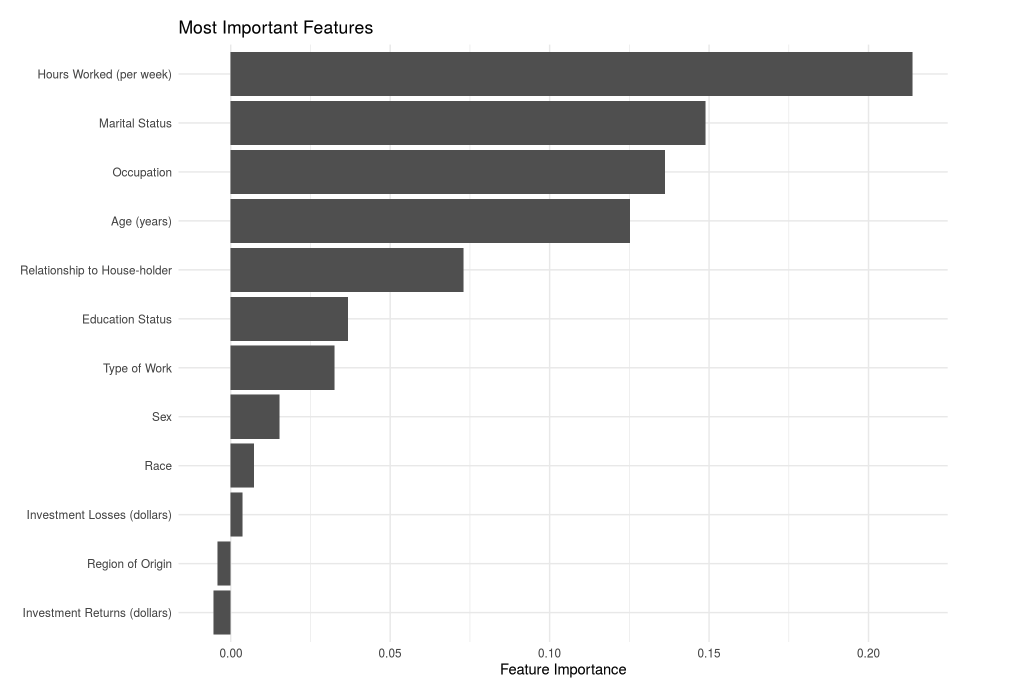
\includegraphics[width=\textwidth]{xai/survey-shap.png}
        \caption{SHAP explanations for \emph{Salary}}
        \label{fig:shapsalary}
    \end{subfigure}
    \hfill
    \begin{subfigure}[b]{0.45\textwidth}
        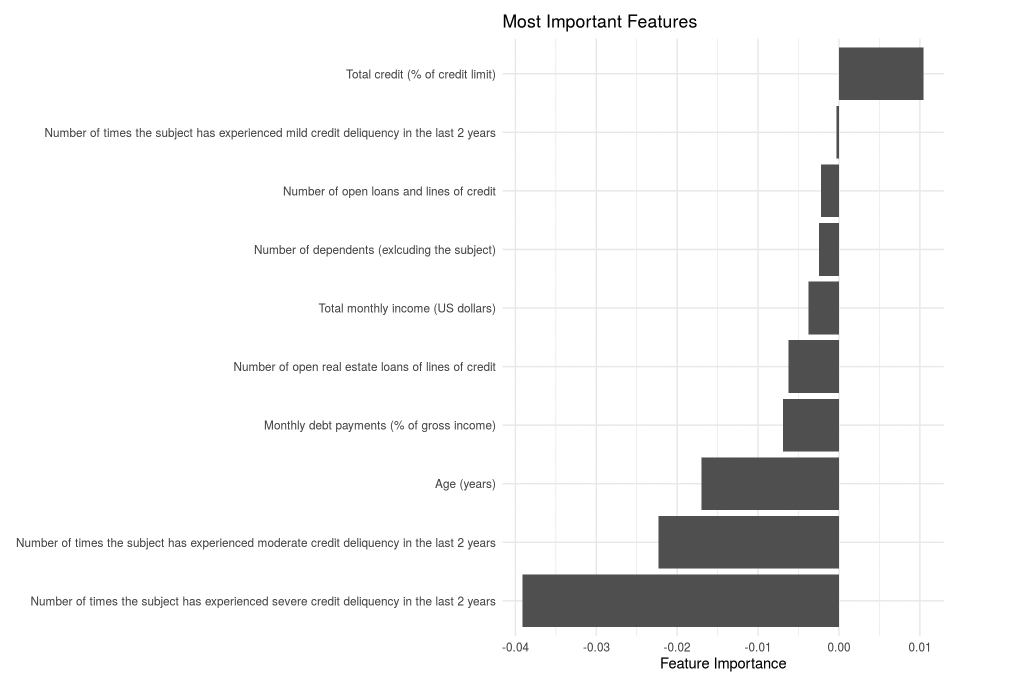
\includegraphics[width=\textwidth]{xai/survey-shap-2.png}
        \caption{SHAP explanations for \emph{Credit}}
        \label{fig:shapcredit}
    \end{subfigure}
    \medskip
    \begin{subfigure}[b]{0.45\textwidth}
        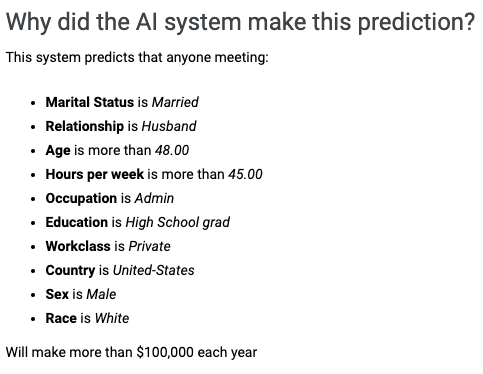
\includegraphics[width=\textwidth]{xai/survey-anchor.png}
        \caption{Anchor explanations for \emph{Salary}}
        \label{fig:anchorsalary}
    \end{subfigure}
    \hfill
    \begin{subfigure}[b]{0.45\textwidth}
        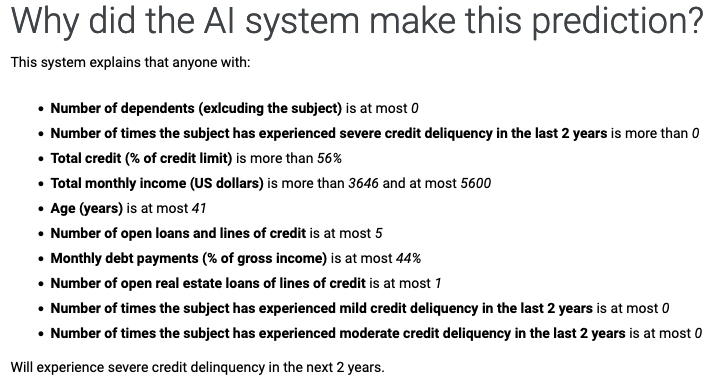
\includegraphics[width=\textwidth]{xai/survey-anchor-2.png}
        \caption{Anchor explanations for $credit$}
        \label{fig:anchorcredit}
    \end{subfigure}
    \medskip
    \begin{subfigure}[b]{0.45\textwidth}
        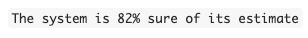
\includegraphics[width=\textwidth]{xai/survey-confidence.png}
        \caption{Confidence explanations for \emph{Salary}}
        \label{fig:confidencesalary}
    \end{subfigure}
    \hfill
    \begin{subfigure}[b]{0.45\textwidth}
        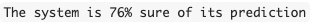
\includegraphics[width=\textwidth]{xai/survey-confidence-2.png}
        \caption{Confidence explanations for \emph{Credit}}
        \label{fig:confidencecredit}
    \end{subfigure}
    \caption{This figure shows sample explanations for all cases. Larger images and more detailed descriptions of explanations can be seen in Appendix \ref{app:figures}.}
    \label{fig:online_explanations}
\end{figure}

\subsubsection{Models}
In both tasks, we construct a predictor model using random forests and augment this predictor with three different explanatory conditions. Our random forest classifier achieves $86\%$ test accuracy on the Adult dataset and $93\%$ test accuracy on the Give Me Some Credit dataset. We use a SHAP explainer to produce one of our explanatory conditions, and an Anchor explainer to produce another; our final explanatory condition is an intrinsic explanation produced by the random forest model. Figure \ref{fig:online_explanations} shows sample explanations produced by these methods. These ultimately form three explanatory conditions: SHAP, Anchor, and Confidence. Note that each participant only receives one model of explanation throughout all 6 cases. 

\subsubsection{Design}
Both tasks rely on the same 3-between-by-2-within design using repeated measures to capture the same data before and after the presentation of each explanation. The between-subjects factor determines which model is used to generate the explanation a given participant will receive. The within-subjects factor is the repeated-measures `explanation presence' factor. This is either `before explanation' or `after explanation', indexed $before$ or $after$. A of the study design can be found in Figure \ref{fig:online_flowchart}.

\begin{figure*}[htbp]
    \centering
    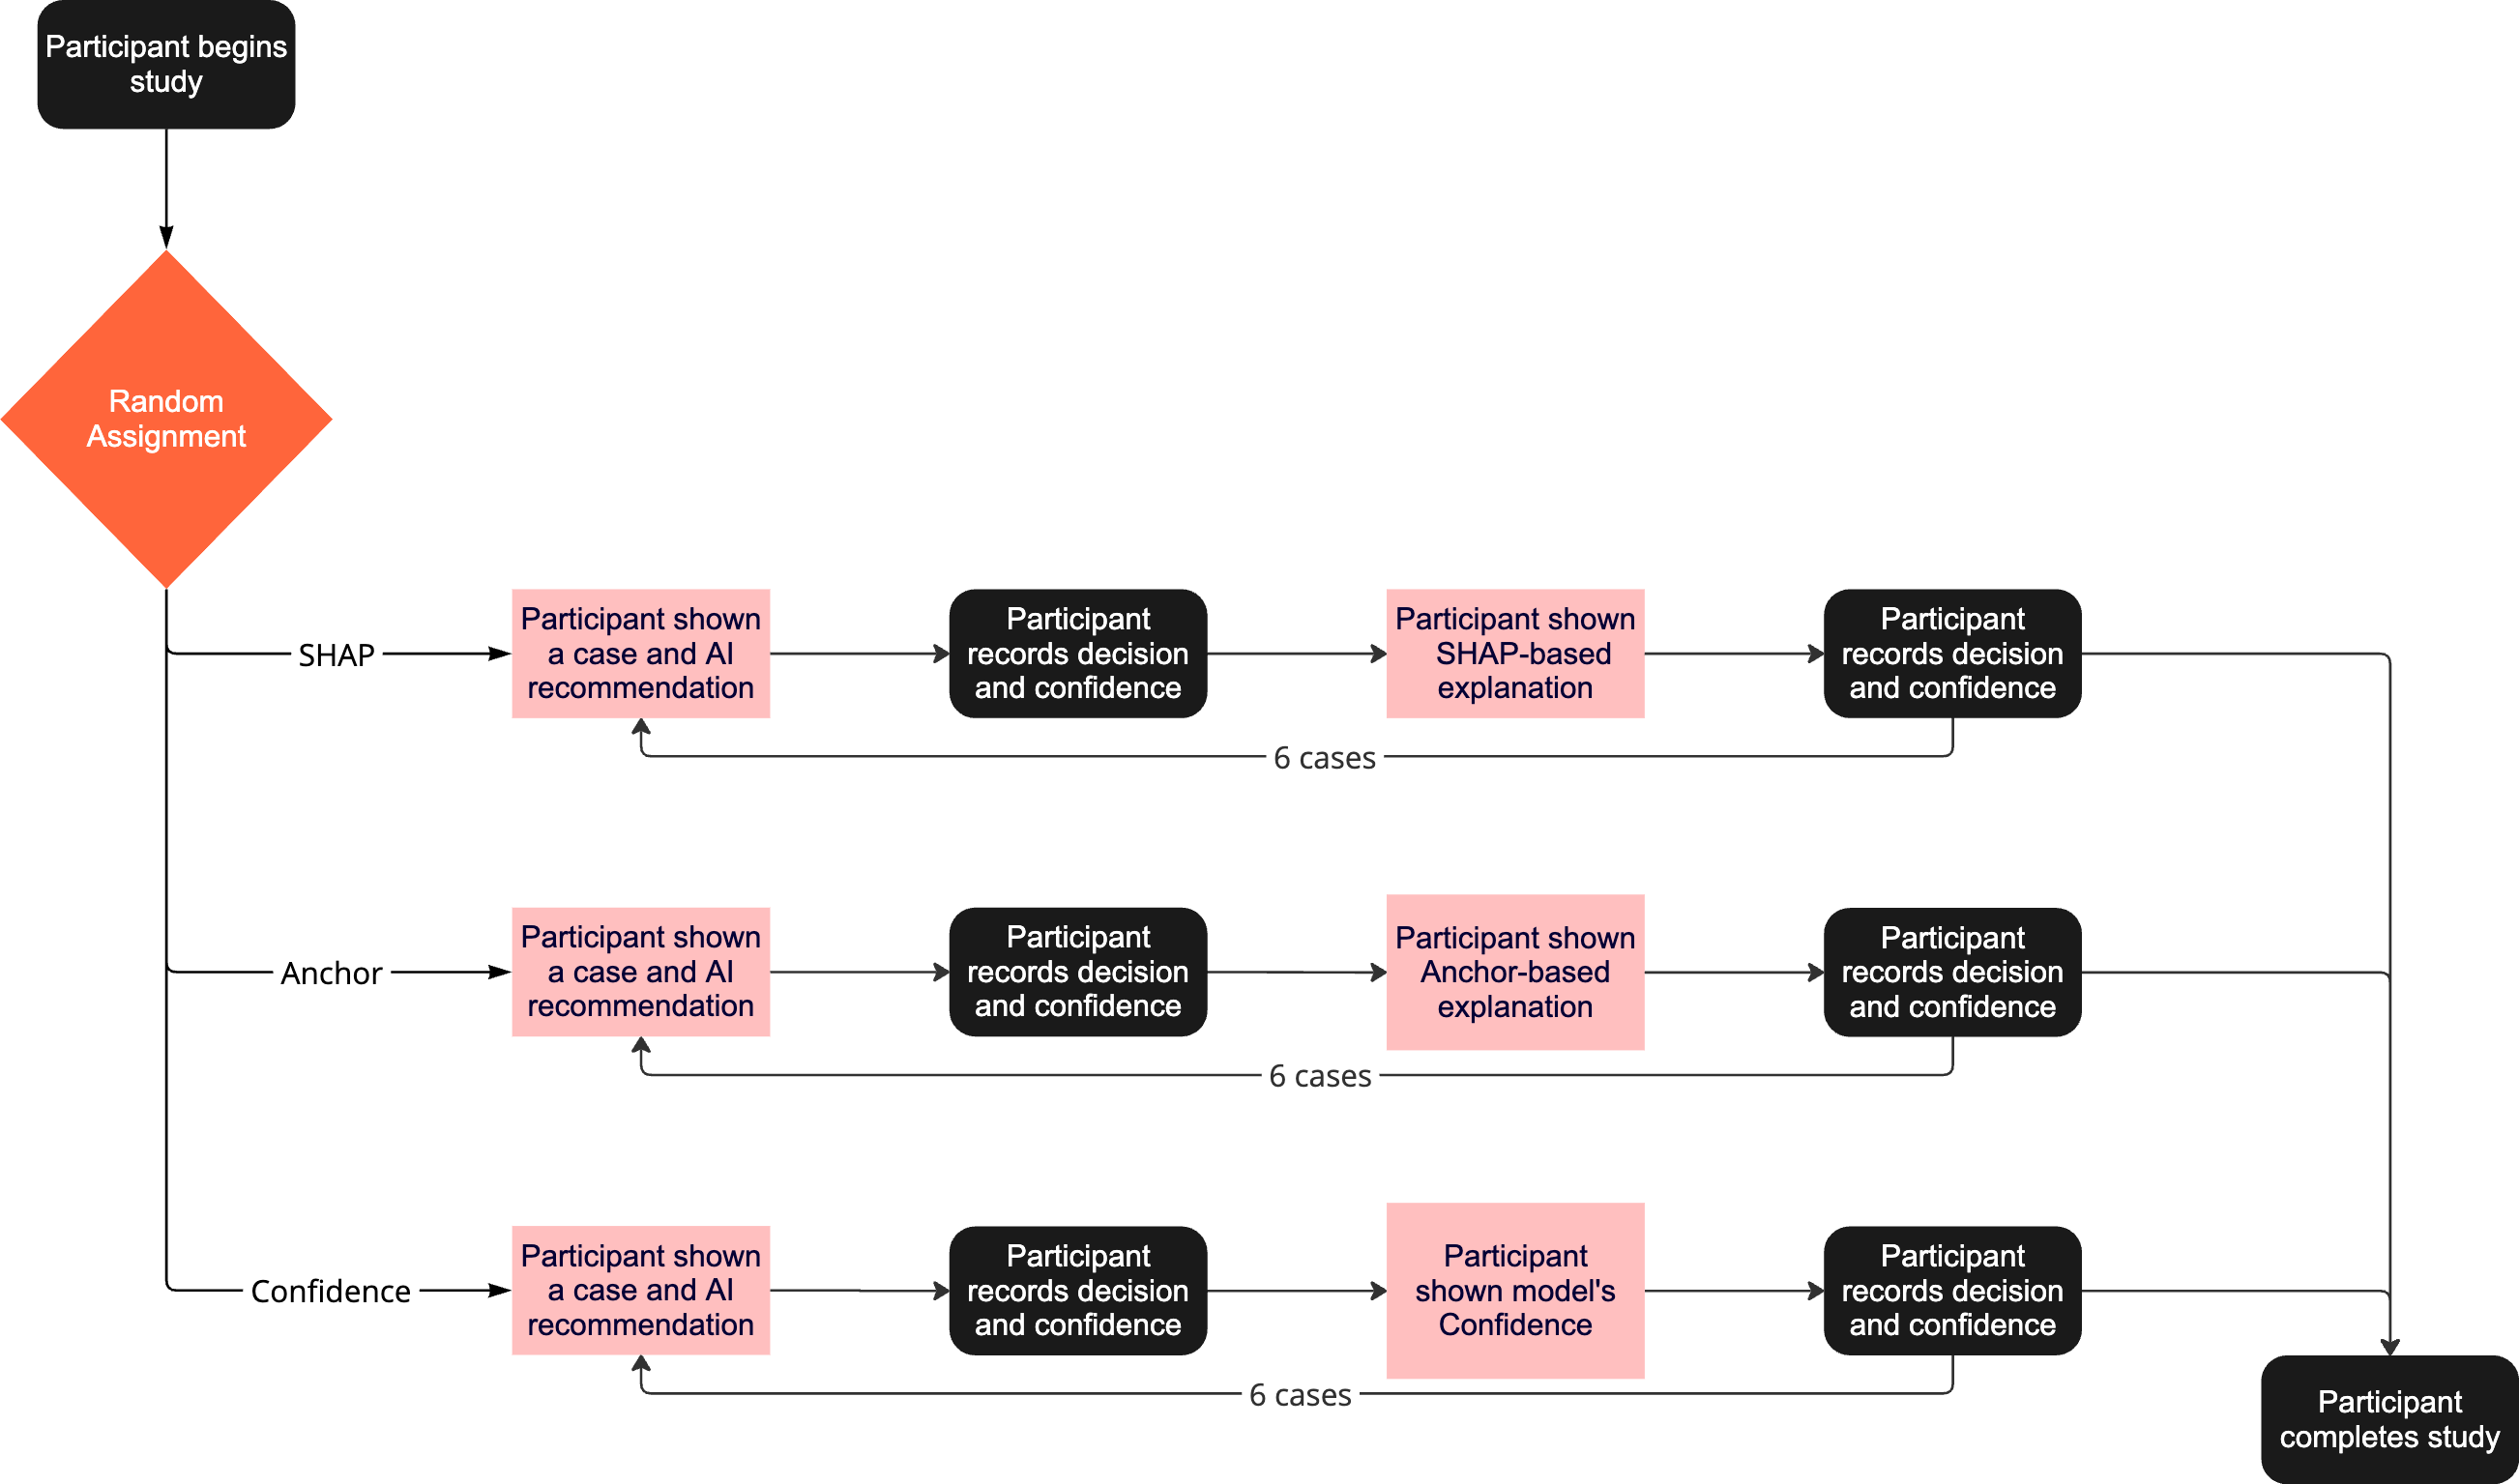
\includegraphics[width=\textwidth]{xai/online_flowchart.png}
    \caption{Participants in the online study are sorted into six buckets, where each bucket is segregated by explanatory condition and task and shown a brief description of the task (i.e., each participant sees only one of the explanations in Figure \ref{fig:online_explanations}). Then, each participant is shown 6 cases. In each case, participants are shown an applicant profile and a AI output. Participants are asked to agree or disagree with the AI output. Then, participants are given explanations based on their explanatory condition scores. They are then asked again to agree or disagree with the AI output.}
    \label{fig:online_flowchart}
\end{figure*}

\subsubsection{Questions and Variables}\label{sssec:q_and_v}
Each participant was shown a brief explanation of the task in question and was then asked to complete the 6 cases, with participants given a random mix of correct and incorrect cases. In each case, participants are first shown a table identifying subject of the case and an AI output of what determination they should make. They are then asked to estimate the dependent variable, and rate both their confidence in the estimate and their trust in the AI output on sliding scales (this is discretised to 20 points).

We code the participant's estimate as a binary $y_{human}$ variable:

\begin{equation}
    y_{human} := \begin{cases}
        \text{How much money do you estimate this person makes?} & (Salary) \\
        \text{Do you predict that this person will experience severe credit delinquency?} & (Credit)
    \end{cases}
\end{equation}

\noindent The two sliding scale responses are coded as $selfconfidence$ and $trust_{attitudinal}$ and have values between 1 and 20. These are defined:

\begin{equation}
    confidence := \begin{cases}
        \text{How confident are you in your estimation?} & (Salary) \\
        \text{How confident are you in your prediction?} & (Credit)
    \end{cases}
\end{equation}

\begin{equation}
    trust_{attitudinal} := \begin{cases}
        \text{How much do you trust the AI's estimation?} & (Salary) \\
        \text{How much do you trust the AI's prediction?} & (Credit)
    \end{cases}
\end{equation}

As we ask all questions in both the $before$ and $after$ conditions, we collect six responses from each participant in each case: $y_{human}^{before}$, $selfconfidence^{before}$, $trust_{attitudinal}^{before}$, $y_{human}^{after}$, $selfconfidence^{before}$, and $trust_{attitudinal}^{after}$.  We additionally have the binary variables $y_{True}$ and $y_{AI}$ that are the true value and the AI output of the dependent variable.

In addition to these, we define $agreement^{before}$ as:

\begin{equation}
    agreement^{before} := \begin{cases}
        1 & \text{if } y_{human}^{before} = y_{AI} \\
        0 & \text{otherwise}
    \end{cases}
\end{equation}

\noindent and $correct_{x}$ as:

\begin{equation}
    correct_{x} := y_{x} = y_{True}
\end{equation}

We define $trust_{behavioural}^{before}$ and $trust_{behavioural}^{after}$ to be the extent to which the participant's confidence agrees with the AI output:

\begin{equation}
    trust_{behavioural}^{x} := \begin{cases}
        confidence^{x}      & \text{if } agreement^{x} \\
        1-confidence^{x}    & \text{otherwise}
    \end{cases}
\end{equation}

Finally, in order to reason about the change in a variable due to the explanation, we define `$\Delta$' constructs for all variables with a $before$ and an $after$ as:

\begin{equation}
    \Delta variable := variable^{after} - variable^{before}
\end{equation}

\noindent so, e.g.:

\begin{equation}
    \Delta trust_{attitudinal} := trust_{attitudinal}^{after} - trust_{attitudinal}^{before}
\end{equation}

\subsubsection{Data Analysis}
We preregistered much of our analyses. Though we also include some post-hoc analysis below, we wish to delineate between the two types of analyses. The former are listed in full here.

We first wish to test for the presence of unwarranted trust. To do this, we measure the difference between ratings in each condition in the cases where the AI output is \textit{incorrect}, i.e. where $\neg correct_{AI}$. To do this, we run three one-sided t-tests \cite{Caldwell-et-al} to determine:

\begin{equation}
    \Delta trust \geq 0 | \neg correct_{AI}
\end{equation}

\noindent for both $\Delta trust_{behavioural}$ and $\Delta trust_{attitudinal}$. Note that this is identical to repeated-measures t-tests on the the $trust_{behavioural}$ and $trust_{attitudinal}$ variables where $\neg correct_{AI}$. Following this, as this is also a between-subjects experiment, we wish to compare the varying effects of different explanation methods in this case. Thus, we run two between-subjects ANOVAs \cite{Caldwell-et-al} on $\Delta trust_{behavioural}$ and $\Delta trust_{attitudinal}$ across the explanatory conditions again filtered on $\neg correct_{AI}$. When these ANOVAs have significant results ($p < 0.05$), we run Tukey's Honestly Significant Difference (HSD) test \cite{Caldwell-et-al}.

Finally, in our Salary Estimation survey, we observed a strong positive correlation between our two trust variables, though we did not preregister it for that study. Indeed, correlation analysis is a well-documented method for confirming two measurements indeed measure the same concept \cite{Westen-and-Rosenthal, Morata-Ramírez-and-Holgado-Tello}. Thus, we additionally included the calculation of Pearson's correlation between $trust_{behavioural}$ and $trust_{attitudinal}$ and between $\Delta trust_{attitudinal}$ and $\Delta trust_{behavioural}$ in our preregistration for the Credit Delinquency Prediction survey. 

\paragraph{Power Analysis}
We run power analyses using \textcite{Caldwell-et-al}'s Superpower. Specifically, we desire sufficiently powerful results on our primary analysis. We select a moderate effect size of interest (Cohen’s $f$) of $0.15$ (yielding group means $-0.15$ and $0.15$ with unit variance), and target a power of at least $0.90$. We note that, using a one-way T-test at $p = 0.05$ and assuming a sample size of $200$, we get power far above $0.90$. We also test for the ANOVA assuming unit variance and group means of $-0.15$, $0.15$, and $0.15$. Under these conditions, we achieve a power of $0.90$ with $200$ samples per condition. We ask each participant a total of 6 questions, and the AI output is incorrect in slightly less than half of them. In order to achieve $200$ samples per condition, therefore, we aim to recruit a total of roughly $66$ participants per condition, or roughly $200$ participants in total.

\paragraph{Preregistration}
We have preregistered analyses for both of our tasks in the OSF registries \cite{natarajan_binns_2022}. 

\subsection{Results}\label{ssec:os_results}
In both tasks, though we originally set $200$ as our target participants, some participants did not complete our task following Prolific Academic's guidelines. Data from these participants was marked incomplete and removed from consideration. 

After this removal, we had a total of $192$ participants complete the Salary Estimation study. These were split randomly into our three explanatory groups. By gender, $115$ were Male, $76$ were Female, and $1$ did not provide gender information. By ethnicity, $137$ were white, $10$ did not provide ethnicity, and the remaining $45$ were split among non-white ethnicities. Our participants were an average of $36.7$ years old, with the youngest being $18$ and the oldest $74$. Each applicant completed an introductory page and six cases. The average completion time for these tasks was $7$ minutes $43$ seconds, the minimum was $2$ minutes $25$, and the maximum was $36$ minutes $46$.

We had a total of $197$ participants complete the Credit Delinquency Prediction study. These were similarly split into groups. By gender, $106$ were Male, $90$ were Female, and $1$ did not provide gender information. By ethnicity, $143$ were white, $11$ did not provide ethnicity, and the remaining $43$ were split among non-white ethnicities. Our participants were an average of $38.4$ years old, with the youngest being $20$ and the oldest $77$. Each applicant completed an introductory page and six cases. The average completion time for these tasks was $7$ minutes $53$ seconds, the minimum was $2$ minutes $17$, and the maximum was $30$ minutes $13$.

\subsubsection{SHAP and Confidence Increase Unwarranted Trust}
We first run the one-sided t-tests on the two trust variables ($attitudinal$ and $behavioural$). I.e., we test:

\begin{equation}
    \Delta trust_{x} > 0 | \neg correct_{AI} \text{ for } x \in \{behavioural, attitudinal\}
\end{equation}

\noindent for both \emph{Salary} and \emph{Credit} across SHAP, Anchor, and Confidence. A positive $F$ statistic here indicates $trust^{after} > trust^{before}$ and a negative $F$ statistic indicates $trust^{after} < trust^{before}$, but, as these are one-sided tests, $p$-values will only be meaningful when $F > 0$. This test was preregistered in both of our tasks \cite{natarajan_binns_2022}. Table \ref{tab:delta-trust-t} contains the results of these analyses.  

\begin{table}[htb]
    \caption{These one-sided t-tests test for $\Delta trust > 0 | \neg correct_{AI}$ for all explanatory conditions and both tasks. We find that SHAP and Confidence increase unwarranted trust in the AI system.}
    \label{tab:delta-trust-t}
    \begin{tabular}{ccccc}
        \toprule
        Task & Explanatory Condition & Variable & F Statistic & p Value \\ 
        \midrule
        Salary Estimation & Anchor & $\Delta trust_{behavioural}$ & $0.509$ & $0.306$ \\
        & & $\Delta trust_{attitudinal}$ & $0.165$ & $0.434$ \\
        & SHAP & $\Delta trust_{behavioural}$ & $\mathbf{3.811}$ & $\mathbf{<0.001}$ \\
        & & $\Delta trust_{attitudinal}$ & $-0.886$ & $0.812$ \\
        & Confidence & $\Delta trust_{behavioural}$ & $\mathbf{2.196}$ & $\mathbf{0.015}$ \\
        & & $\Delta trust_{attitudinal}$ & $0.945$ & $0.173$ \\
        \midrule
        Credit Delinquency Prediction & Anchor & $\Delta trust_{behavioural}$ & $1.396$ & $0.082$ \\
        & & $\Delta trust_{attitudinal}$ & $-2.364$ & $0.990$ \\
        & SHAP & $\Delta trust_{behavioural}$ & $1.516$ & $0.066$ \\
        & & $\Delta trust_{attitudinal}$ & $\mathbf{2.475}$ & $\mathbf{0.007}$ \\
        & Confidence & $\Delta trust_{behavioural}$ & $\mathbf{1.835}$ & $\mathbf{0.034}$ \\
        & & $\Delta trust_{attitudinal}$ & $0.940$ & $0.174$ \\
        \bottomrule
    \end{tabular}
\end{table}

This indicates that SHAP and Confidence appear to lead users to trust the AI system more when that system is wrong. We find this result more strongly for behavioural trust than attitudinal trust in all but one test.

Notably, Anchor does not follow this pattern, and instead shows no significant increase in either attitudinal or behavioural trust on these one-sided t-tests. (However, as we explore in Section \ref{sec:anchor-attitudinal}, they may show a significant decrease.)

\subsubsection{Different Explanation Styles Have Different Effects on Unwarranted Trust}
We have shown already that SHAP and Confidence induce unwarranted trust relative to no explanation; we now show that there is significant difference in the effect of some explanatory conditions relative to others. To do this, we examine the $\Delta trust_{behavioural}$ and $\Delta trust_{attitudinal}$ variables across explanatory conditions with an ANOVA test. For this test, we filter on $\neg correct_{AI}$. I.e.:

\begin{equation}
    \Delta \text{ any}(trust_{x1,x2} \neq trust_{x1,x3}) | \neg correct_{AI} \text{ for } x1 \in \{behavioural, attitudinal\} \text{ and } x2,x3 \in \{SHAP, Anchor, Confidence\}
\end{equation}

\noindent This test was preregistered in both of our tasks \cite{natarajan_binns_2022}. Table \ref{tab:delta-trust-anova} contains the results of these analyses.

\begin{table}[htb]
    \caption{These ANOVAs compare $\Delta trust$ between SHAP, Confidence, and Anchor to indicate where significant differences exist. We find two statistically significant differences, indicating that we should focus post-hoc analyses on these two.}
    \label{tab:delta-trust-anova}
    \begin{tabular}{lrrr}
        \toprule
        Task & Variable & F Statistic & p Value \\
        \midrule
        Salary Estimation & $\Delta trust_{behavioural}$ & $\mathbf{3.671}$ & $\mathbf{0.026}$ \\
        & $\Delta trust_{attitudinal}$ & $0.925$ & $0.397$ \\
        \midrule
        Credit Delinquency Prediction & $\Delta trust_{behavioural}$ & $0.066$ & $0.936$ \\
        & $\Delta trust_{attitudinal}$ & $\mathbf{6.213}$ & $\mathbf{0.002}$ \\
        \bottomrule
    \end{tabular}
\end{table}

Note from Table \ref{tab:delta-trust-anova} that in the Salary Estimation task, we find no significant results for our ANOVA $trust_{attitudinal}$, but do find significant results for $trust_{behavioural}$. However, in the Credit Delinquency Prediction task, we find significant results for our ANOVA $trust_{attitudinal}$, but none for $trust_{behavioural}$. We examine these two findings separately.

\subsubsection{SHAP Increases Behavioural Trust More than Anchor in the Salary Estimation Task}
We now show that:

\begin{equation}
    \Delta trust_{behavioural,SHAP,salary} > \Delta trust_{behavioural,Anchor,salary} | \neg correct_{AI}
\end{equation}

\noindent Note that, while the result of the ANOVA test in table \ref{tab:delta-trust-anova} supports that there is indeed a statistically significant difference in the three group means of the $\Delta trust_{behavioural}$ variable, it does not specify which means are greater and which are less. For an indication of which means are greater, following our preregistered protocol for significant ANOVA results, we turn to Tukey's Honestly Significant Difference (HSD) test as a post-hoc test in table \ref{tab:delta-trust-hsd}. As we found significant results in the ANOVA test of $\Delta trust_{behavioural}$ filtered on $\neg correct_{AI}$, we restrict our post-hoc analysis to this variable.

\begin{table}[htb]
    \caption{Tukey's HSD test compares $\Delta trust_{behavioural,x}$ in \emph{Salary} with $\neg correct_{AI}$. We find that SHAP increases behavioural trust in incorrect AI outputs more than Anchor.}
    \label{tab:delta-trust-hsd}
    \begin{tabular}{lllrr}
        \toprule
        Explanatory Condition A & Explanatory Condition B & Variable & Test Statistic & p Value \\
        \midrule
        SHAP & Anchor & $\Delta trust_{behavioural}$ & $\mathbf{2.310}$ & $\mathbf{0.022}$ \\
        Confidence & Anchor & $\Delta trust_{behavioural}$ & $0.855$ & $0.599$ \\
        SHAP & Confidence & $\Delta trust_{behavioural}$ & $1.455$ & $0.198$ \\
        \bottomrule
    \end{tabular}
\end{table}

As can be seen in Table \ref{tab:delta-trust-hsd}, we observe a significant difference in the mean of $\Delta trust_{behavioural}$ between the SHAP and Anchor conditions with $\neg correct_{AI}$, but we do not observe a significant difference between the other conditions. This indicates that, beyond increasing behavioural trust in incorrect AI outputs, SHAP increases behavioural trust in incorrect AI outputs \emph{more} than Anchor.

\subsubsection{Anchor Decreases Unwarranted Attitudinal Trust Relative to SHAP and Confidence in the Credit Delinquency Prediction Task}
Note that we found a large negative F for $\Delta trust_{attitudinal}$ in the Anchor case in the Credit Delinquency Prediction portion of table \ref{tab:delta-trust-t} – an effect that is not significant due to the one-sidedness of our tests. However, as we found only positive F values for $\Delta trust_{attitudinal}$ in the SHAP and Confidence cases, we might expect that Anchor has a negative effect on $\Delta trust_{attitudinal}$ relative to SHAP and Confidence. Indeed, the result of the ANOVA test in table \ref{tab:delta-trust-anova} supports that there is indeed statistically significant difference in the three group means of the $\Delta trust_{attitudinal}$ variable in this task, though it again does not specify which groups are different, or how.

For an indication of which means are greater, following our preregistered protocol for significant ANOVA results, we turn again to a Tukey's HSD test as a post-hoc test in table \ref{tab:delta-trust-hsd-2}. As we found significant results in the ANOVA test of $\Delta trust_{attitudinal}$ filtered on $\neg correct_{AI}$, we restrict our post-hoc analysis to this variable. We test:

\begin{equation}
    \Delta trust_{behavioural,x1,credit} > \Delta trust_{behavioural,x2,credit} | \neg correct_{AI} for x1,x2 \in \{SHAP, Anchor, Confidence\}
\end{equation}

\begin{table}[htb]
    \caption{Tukey's HSD test compares $\Delta trust_{attitudinal}$ across explanations in \emph{Credit} with $\neg correct_{AI}$. We find that Anchor decreases unwarranted trust relative to SHAP and Confidence.}
    \label{tab:delta-trust-hsd-2}
    \begin{tabular}{lllrrc}
        \toprule
        Explanatory Condition A & Explanatory Condition B & Variable & Test Statistic & p Value \\
        \midrule
        SHAP & Anchor & $\Delta trust_{attitudinal}$ & $\mathbf{1.213}$ & $\mathbf{<0.001}$ \\
        Confidence & Anchor & $\Delta trust_{attitudinal}$ & $\mathbf{1.030}$ & $\mathbf{<0.001}$ \\
        SHAP & Confidence & $\Delta trust_{attitudinal}$ & $0.183$ & $0.708$ \\
        \bottomrule
    \end{tabular}
\end{table}

As can be seen in table \ref{tab:delta-trust-hsd-2}, we observe a significant difference in the mean of $\Delta trust_{behavioural}$ between the Anchor condition and both other conditions, but we do not observe a significant difference between SHAP and Confidence. This indicates that, relative to both other conditions, Anchor actually \emph{reduces} attitudinal trust in the AI output.

Note that this does not prove that Anchor reduces attitudinal trust relative to no explanation. For this analysis, we will need another t-test. As we did not preregister this test, analysis of this phenomenon is included in exploratory analysis below.

\subsubsection{Behavioural and Attitudinal Trust are Highly Correlated}
It should be noted that some patterns observed for $trust_{behavioural}$ do not hold for $trust_{attitudinal}$ and vice-versa. However, while they are mathematically distinct constructs, they are both intended to measure the same underlying phenomenon. We apply Pearson's correlation analysis across all explanatory conditions in both the before- and after- cases. We also perform this analysis on $\Delta trust_{attitudinal}$ and $\Delta trust_{behavioural}$. 

For this analysis, we do not filter out positive cases. Rather, we consider all cases together. Results can be seen in table \ref{tab:trust-correlation}.\footnote{This analysis was only partially preregistered; we did not register this analysis in the Salary Estimation task, but we did in the Credit Delinquency Prediction task \cite{natarajan_binns_2022}.}

\begin{table}[htb]
    \caption{Pearson's test shows a high correlation between $trust_{attitudinal}$ and $trust_{behavioural}$ in both tasks. This correlation extends to the relationship between $\Delta trust_{attitudinal}$ and $\Delta trust_{behavioural}$.}
    \label{tab:trust-correlation}
    \begin{tabular}{lllrr}
        \toprule
        Task & Variable A & Variable B & Rho & p \\
        \midrule
        Salary Estimation & $trust_{attitudinal}$ & $trust_{behavioural}$ & $\mathbf{0.630}$ & $\mathbf{<0.001}$ \\
        & $\Delta trust_{attitudinal}$ & $\Delta trust_{behavioural}$ & $\mathbf{0.265}$ & $\mathbf{<0.001}$ \\
        \midrule
        Credit Delinquency Prediction & $trust_{attitudinal}$ & $trust_{behavioural}$ & $\mathbf{0.612}$ & $\mathbf{<0.001}$ \\
        & $\Delta trust_{attitudinal}$ & $\Delta trust_{behavioural}$ & $\mathbf{0.179}$ & $\mathbf{<0.001}$ \\
        \bottomrule
    \end{tabular}
\end{table}

Note that, though the attitudinal and behavioural variables display different behaviour in other analyses, table \ref{tab:trust-correlation} indicates that they are indeed highly correlated across both of our tasks. Furthermore, though the correlation between the $\Delta trust$ is more modest, it is still statistically significant. These together leave little doubt that $trust_{attitudinal}$ and $trust_{behavioural}$ measure related, and perhaps even identical, concepts. In other words, when a participant says they trust the AI output, they generally act accordingly.

\subsubsection{Anchor Decreases Attitudinal Trust in AI Outputs}\label{sec:anchor-attitudinal}
Having found no significant result indicating the presence of the hypothesised effect of Anchor explanations on unwarranted trust, we explore what effect Anchor explanations have on end users' trust in incorrect AI outputs. For the purposes of this analysis, we filter on $\neg correct_{AI}$.\footnote{This analysis was not preregistered.}

We noted already that SHAP and Confidence appear to increase trust in cases where the AI output is incorrect. However, we noticed no such result for Anchor. However, we did observe an apparent negative effect on $\Delta trust_{attitudinal}$ in the t-tests for the Credit Delinquency Prediction task, though, as the tests were one-sided, we could not confirm significance. Thus, we repeat this test as a two-sided test, as shown in table \ref{tab:delta-trust-t-2}. We also repeat other t-tests on Anchor as two-sided, though, as they all have positive F-values, note that none can yield significant results.

\begin{table}[htb]
    \caption{Two-sided t-tests compare $\Delta trust_{x,Anchor} \neq 0 for x \in \{attitudinal, behavioural\}$ in both tasks. We find that Anchor explanations decrease attitudinal trust in incorrect AI outputs in \emph{Credit}, but all other results are inconclusive.}
    \label{tab:delta-trust-t-2}
    \begin{tabular}{lllrr}
        \toprule
        Task & Explanatory Condition & Variable & t Statistic & p Value \\ 
        \midrule
        Salary Estimation & Anchor & $trust_{behavioural}$ & $0.509$ & $0.611$ \\
        & & $trust_{attitudinal}$ & $0.165$ & $0.869$ \\
        \midrule
        Credit Delinquency Prediction & Anchor & $trust_{behavioural}$ & $1.396$ & $0.164$ \\
        & & $trust_{attitudinal}$ & $\mathbf{-2.364}$ & $\mathbf{0.019}$ \\
        \bottomrule
    \end{tabular}
\end{table}

Note here that, on the two-sided t-test, we \textit{do} find a that the provision of Anchor explanations decreases participant attitudinal trust in incorrect AI output, at least in the Credit Delinquency Prediction task. However, we do not see a similar effect on behavioural trust. 

\subsubsection{Anchor and SHAP Increase Participant Self-Confidence in their Determinations}
Noting that behavioural trust is an index variable constructed from $selfconfidence$, we ask: does providing an Anchor explanation increase participant confidence in their own decisions when the AI output is incorrect? Similarly, we ask this question for both the SHAP and Confidence conditions, following exactly the format of the preregistered one-sided t-tests in table \ref{tab:delta-trust-t}, but applied to the variable $\Delta selfconfidence$. Again, we filter on $\neg correct_{AI}$.:

\begin{equation}
    \Delta selfconfidence > 0 | \neg correct_{AI}
\end{equation}

Analysis can be seen in table \ref{tab:delta-confidence-t}.\footnote{This analysis was not preregistered.} Note for clarity that $selfconfidence$ is the variable indicating participant confidence in their own decisions, and Confidence is the condition in which the explanation consists of the AI's own confidence in its suggestion.

\begin{table}[htb]
    \caption{One-sided t-tests determine whether $\Delta selfconfidence > 0$ where $\neg correct_{AI}$ for all explanatory conditions and both tasks. We find that Anchor and SHAP increase participant self-confidence in their determinations, while Confidence yields inconclusive results.}
    \label{tab:delta-confidence-t}
    \begin{tabular}{lllrr}
        \toprule
        Task & Explanatory Condition & Variable & t Statistic & p \\
        \midrule
        Salary Estimation & Anchor & $selfconfidence$ & $\mathbf{2.171}$ & $\mathbf{0.016}$ \\
        & SHAP & $selfconfidence$ & $\mathbf{1.694}$ & $\mathbf{0.046}$ \\
        & Confidence & $selfconfidence$ & $1.047$ & $0.296$ \\
        \midrule
        Credit Prediction & Anchor & $selfconfidence$ & $\mathbf{1.742}$ & $\mathbf{0.042}$ \\
        & SHAP & $selfconfidence$ & $\mathbf{3.473}$ & $\mathbf{<0.001}$ \\
        & Confidence & $selfconfidence$ & $0.752$ & $0.226$ \\
        \bottomrule
    \end{tabular}
\end{table}

We note that, while Confidence shows no significant effects on either task, participants shown an Anchor or SHAP explanation grow significantly more confident in their prediction, indicating that providing an Anchor or SHAP explanation serves to increase a participant's confidence in their \emph{own estimate}.

\subsubsection{Explanations Impact Trust Differently When the AI Output is Correct}
Note that ideally calibrated trust would involve both distrusting the AI output when it is wrong and trusting it when it is right. To assess the latter, we now turn to an evaluation of what happens in the cases where the AI is correct, i.e. $correct_{AI}$. Namely, we conduct two-sided t-tests on both trust variables in all three cases. Table \ref{tab:delta-trust-t-positives} contains the results of these analyses.\footnote{These analyses were not preregistered.}

\begin{table}[htb]
    \caption{These two-sided t-tests compare $\Delta trust$ when $correct_{AI}$. We find that Confidence and SHAP increase trust in the AI system when it is correct, while Anchor decreases attitudinal trust in the AI system, but increases behavioural trust.}
    \label{tab:delta-trust-t-positives}
    \begin{tabular}{lllrr}
        \toprule
        Task & Explanatory Condition & Variable & t Statistic & p Value \\ 
        \midrule
        Salary Estimation & Anchor & $trust_{behavioural}$ & $0.502$ & $0.616$ \\
        & & $trust_{attitudinal}$ & $\mathbf{-2.337}$ & $\mathbf{0.020}$ \\
        & SHAP & $trust_{behavioural}$ & $0.295$ & $0.768$ \\
        & & $trust_{attitudinal}$ & $-1.385$ & $0.168$ \\
        & Confidence & $trust_{behavioural}$ & $\mathbf{2.410}$ & $\mathbf{0.017}$ \\
        & & $trust_{attitudinal}$ & $\mathbf{3.254}$ & $\mathbf{0.001}$ \\
        \midrule
        Credit Delinquency Prediction & Anchor & $trust_{behavioural}$ & $\mathbf{3.013}$ & $\mathbf{0.003}$ \\
        & & $trust_{attitudinal}$ & $\mathbf{-2.487}$ & $\mathbf{0.014}$ \\
        & SHAP & $trust_{behavioural}$ & $0.207$ & $0.836$ \\
        & & $trust_{attitudinal}$ & $\mathbf{3.538}$ & $\mathbf{0.001}$ \\
        & Confidence & $trust_{behavioural}$ & $\mathbf{2.863}$ & $\mathbf{0.005}$ \\
        & & $trust_{attitudinal}$ & $\mathbf{2.461}$ & $\mathbf{0.015}$ \\
        \bottomrule
    \end{tabular}
\end{table}

\paragraph{Confidence Explanations Increase Warranted Trust}
Note that, for both trust variables and both tasks, the Confidence condition boasts a significant positive $\Delta trust$. In other words, when the AI output is correct, providing its confidence in its own prediction increases both behavioural and attitudinal trust towards the AI.

\paragraph{Anchor Explanations Decrease Warranted Attitudinal Trust but Increase Warranted Behavioural Trust}
In the Anchor case, it is clear that providing Anchor explanations yields a large decrease in $trust_{attitudinal}$. This, along with the finding that Anchor explanations decrease $trust_{attitudinal}$ when $\neg correct_{AI}$, would indicate that Anchor explanations have an overall negative impact on $trust_{attitudinal}$, regardless of case. Despite this, providing Anchor explanations yields an increase in $trust_{behavioural}$ (though this is only significant in the \emph{Credit} case). This suggests that, though participants report lower trust in AI outputs when shown an Anchor explanation, they behave as though their trust in the outputs is appropriately calibrated.\footnote{Though $trust_{attitudinal}$ and $trust_{behavioural}$ are closely correlated overall, this represents one instance in which they appear to reveal differences in participant behaviour.}

\paragraph{SHAP Explanations Increase Warranted Attitudinal Trust in the Credit Delinquency Prediction Task}
In the SHAP case, we find a large significant positive $F$ for $trust_{attitudinal}$ when $correct_{AI}$ in the credit delinquency prediction task. However, not only is the effect not mirrored in either tests of $trust_{behavioural}$, but the same test on the salary estimation task actually has a negative $F$ value.

\subsection{Study Findings}\label{ssec:os_discussion}
Our results indicate that both SHAP and Confidence induce unwarranted trust in the explainee. I.e., on the \emph{Salary} and \emph{Credit} tasks, neither SHAP nor Confidence serve to correctly calibrate trust in AI outputs. Rather, they blindly increase trust in these outputs, encouraging users to incorrectly agree with the AI outputs. While this confirms the cautionary critique of \textcite{Lipton} as applied to SHAP in our domain, our results relating to Confidence suggest this critique is too narrow. Namely, issues of unwarranted trust do not seem confined to post-hoc xAI, but are rather a function of providing post-hoc justification of the model's output. This suggests that even un-optimised notions of interpretability, when provided post-hoc as justifications of model outputs, induce unwarranted trust.

Challenging this interpretation, we find no similar effect for Anchor. Instead, we find a significant decrease in participants' stated confidence in AI and a simultaneous increase in participant self-confidence in their own decisions. \textcite{Miller} identifies a number of features that social sciences would suggest make a good explanation; we conclude, following Section \ref{ssec:history}, that Anchor explanations serve to highlight strange model behaviour that correctly undermines explainee confidence in model outputs. In short, the problem is not the use of explanations as justification tools, but rather the use of ``bad'' explanations as justification tools.

This raises another question: if SHAP and Confidence are ``bad'' explanations as \emph{in-process} justification tools, are they ``good'' explanations for something else?

\section{Participatory Design: \emph{Ex-Post} Decision Support}\label{sec:case}
\subsection{Motivation}
In Section \ref{sec:online}'s investigation of post-hoc explainable AI, we found that SHAP-based explanations, in particular, can lead to unwarranted trust when used to justify decisions. It is clear, at least, that we should not use SHAP-based explanations as a DST in this context. However, we do not suggest that SHAP should be discarded entirely. In fact, though \emph{Salary} and \emph{Credit} both prove unsuitable tasks for applications of SHAP-based explanations as DSTs, we suggest that we might still make use of the explanations. In particular, in use cases where explainee trust in the underlying model is not at issue, SHAP's induction of unwarranted trust need not undermine its utility.

It is clear that when making a `primary' decision (i.e., the same decision the model output seeks to make), human reviewers working from AI outputs are preeminently concerned with whether to agree with or overrule the model's output. However, after making this decision, they are no longer necessarily concerned with whether to agree or disagree with the model's output. Consider the task of \emph{refining a scholarship selection algorithm}, the \emph{Refinement} task. Scholarship and talent investment programs ordinarily select cohorts in a series of application cycles \cite{li2020hiring}. Between application cycles, they seek to examine their previous selection decisions, and possibly modify their processes to improve these decisions in the future \cite{li2020hiring}; if AI algorithms are used to support these decisions, the review will naturally include refinements to the AI algorithms. In this case, though, we are no longer concerned with whether the AI was correct; rather, we are concerned with whether the way the AI informs decision-making is conducive to ideal selection pipelines.

We conducted a human-centric study using SHAP explanations as an \emph{ex-post} explanation tool to help selection practitioners from a scholarship and talent investment program with the \emph{Refinement} task. Through this participatory design study, we assess SHAP's usefulness based on the insights these explanations provide.

This study aims to answer RQ2:

\begin{enumerate}
    \item[(RQ2)] If post-hoc xAI methods induce unwarranted trust \emph{in-process}, could they still be useful \emph{ex-post}?\footnote{Recall the distinction between \emph{ex-post} and post-hoc. We use the term `post-hoc' to refer to explanation algorithms that are applied after a model; \emph{ex-post}, in contrast, refers to the explanation tools applied in decision support scenarios where the primary decisions have already been made.}
\end{enumerate}

\noindent In doing so, we restrict our attention specifically to SHAP, as we have already demonstrated its induction of unwarranted trust.

\subsection{Methodology}\label{ssec:cs_methods}
We test SHAP's usefulness in a human-centred context. To do so, we run a study with scholarship and talent investment selection practitioners (N=8) from a scholarship and talent investment organisation. Though the organisation already uses algorithmic scoring to support their decision-making, no practitioners possess experience with post-hoc xAI prior to the study. The study consists of two participatory design workshops with said practitioners – we term these `G1' and `G2'.\footnote{to preserve the anonymity of the participants, we do not number or identify participants. Rather, we attribute quotes based on workshop group.}

Before this study, we obtained informed consent from all participants. As we run group workshops (and as we do not attribute comments to individual participants), participants were informed that they would not be able to recuse themselves after the study. Participants also gave consent to be recorded, and to have these recordings stored on a secure server. All recording, transcribing, and data analysis was conducted on secure servers. Ethics review was performed by University of Oxford's Central University Research Ethics Committee.

\begin{figure}[htbp]
    \centering
    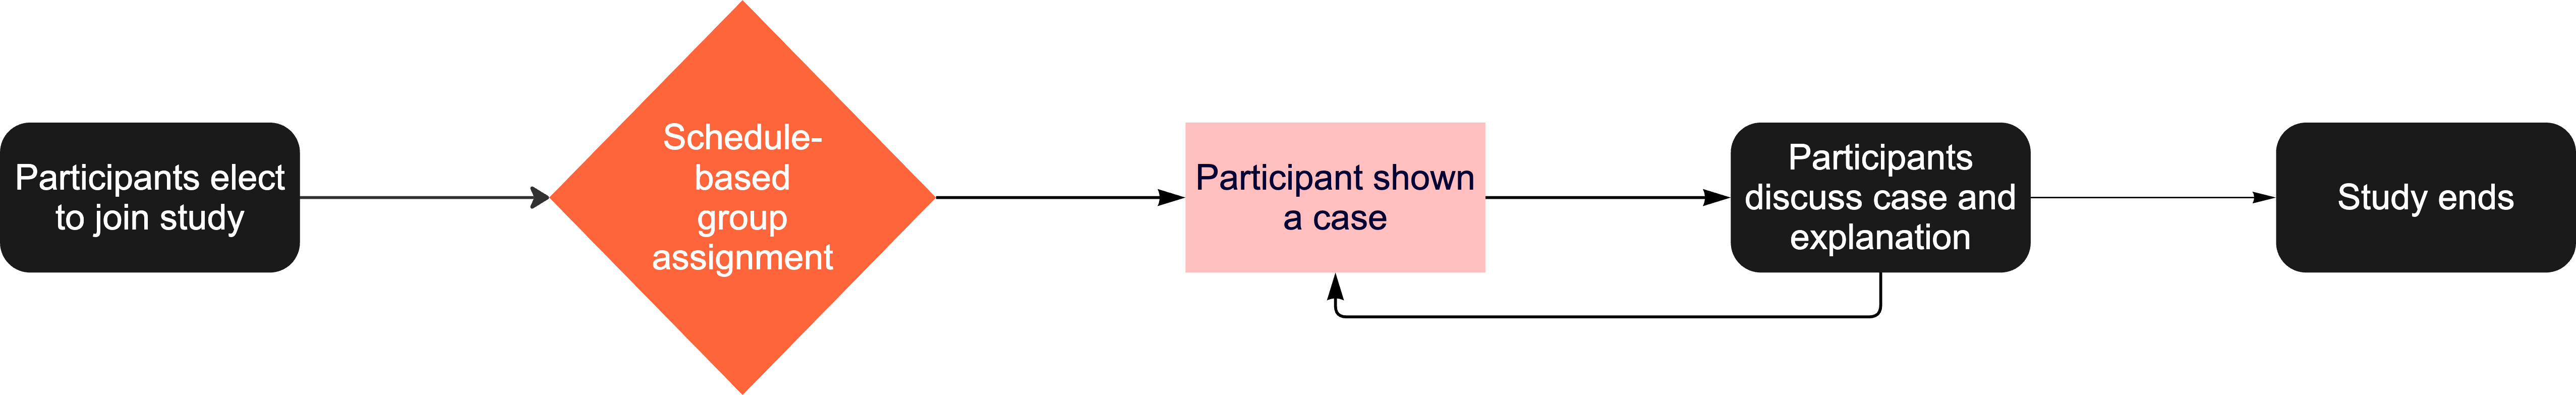
\includegraphics[width=.9\textwidth]{xai/case_flowchart.png}
    \caption{Each workshop consists of a series of cases relating to a past application decision that was flagged by program reviewers. In each case, participants are shown slides like in Figure \ref{fig:sample_case} and are asked to analyse the algorithm itself and whether the case warrants changes to the algorithm in future years.}
    \label{fig:case_flowchart}
\end{figure}

Both workshops followed an identical protocol. The flow of these workshops is shown in Figure \ref{fig:case_flowchart}, and more detail on the protocol followed can be found in Appendix \ref{app:protocol}.

In each workshop, participants discussed a number of cases, each examining a (possibly successful) applicant from a past application cycle who was flagged by program reviewers for having perplexing algorithm scores relative to other known information. In each case, participants are asked to use visual, SHAP-based explanations to first understand why program reviewers found these cases worth noting, then to explore why program reviewers gave the feedback they did and what caused the algorithm's perplexing outputs, and finally to opine on whether the case suggests that changes should be made to the algorithm (or to the selection process as a whole) for future years. The cases themselves have been redacted, as they contain sensitive information about program applicants, but a sample case can be seen in Figure \ref{fig:sample_case}.

In analysing our data, we follow \textcite{braun_using_2006}'s methodology for reflexive thematic analysis. 

\begin{figure}[htbp]
    \centering
    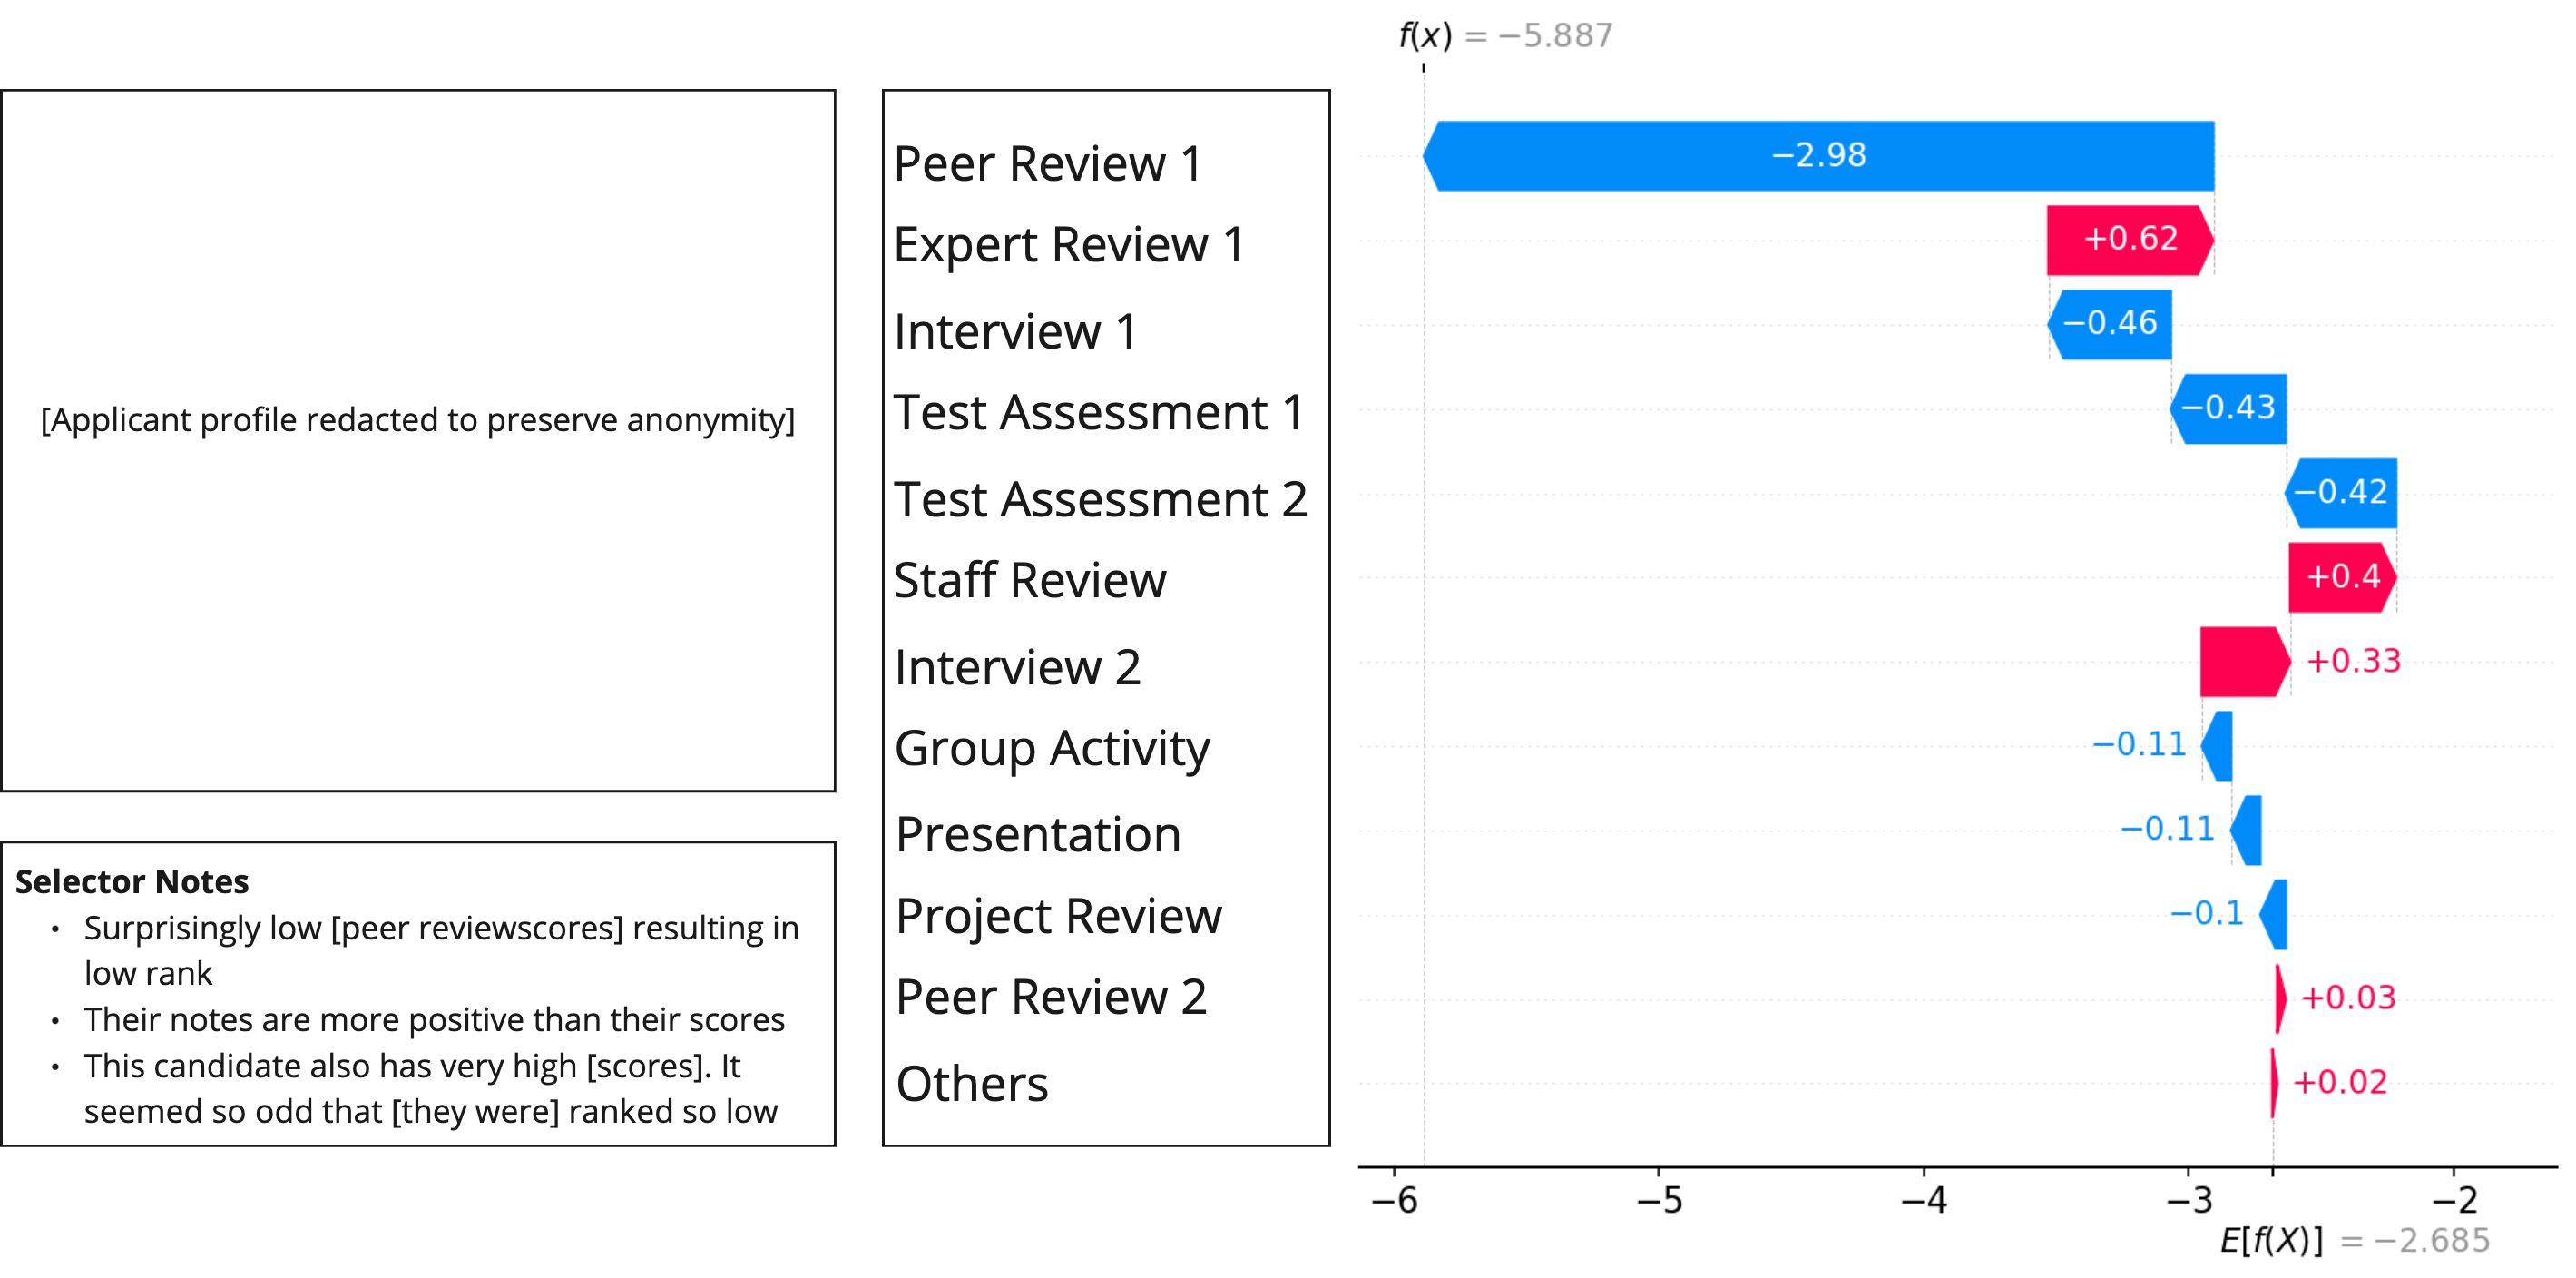
\includegraphics[width=.9\textwidth]{xai/sample_case.png}
    \caption{Each case explores one applicant from past years chosen by past program reviewers after being flagged as having perplexing algorithm scores. Each case contains the applicant's profile (overall algorithm scores alongside demographic information; the profile is redacted to preserve applicant anonymity), the program reviewers' comments, and the SHAP-based explanation (the score names are replaced with generic labels to preserve program anonymity).}
    \label{fig:sample_case}
    
\end{figure}

\subsection{Results}\label{sec:cs_results}
Our case study yielded two key themes. Firstly, SHAP Explanations yield useful \emph{ex-post} insights about feature importance. Second, even though SHAP yields useful information, the accessibility of such information depends on careful presentation. We now cover these in depth.

\subsubsection{Ex-Post Insights on Important Features}
In both groups, several useful insights emerged due to the SHAP visualisations. For example, the relationships between scores and contextual factors (e.g., markers of applicants' socioeconomic status) revealed that context plays little to no role in scoring; despite this, an applicant's context has a strong impact on how selection practitioners read scores. E.g., an applicant with high test scores from a poor region of Kenya is more impressive than one with high test scores from a rich part of the United Kingdom. When discussing one applicant who was selected, but had particularly low algorithmic scores, one participant said: ``This is one of the candidates that... [was from a] different country and [had] very low income'' (G1). Such cases raise difficult questions about fairness, including whether markers of disadvantage should be factored into decision-making, or if decision-makers should focus only on `task-relevant' factors \cite{dwork_fairness_2012}. If algorithms aren't taking into account such information, we are all but guaranteed to find discrepancies between algorithmically-driven selections and human-made ones.

It was also remarked on that scores calculated based on the feedback of external experts often disagreed with scores calculated based on the feedback of program applicants. It was discovered here that, contrary to program expectations, the program's expert reviews appeared less prone to biases than the peer ones. For one applicant: ``There was a question about why his peer and expert review were so different...I think confirms that it's not actually that they were seeing dramatically different things...his peers were dinging him for not seeming like he needed the award'' (G1). For another: ``I think this applicant has been significantly brought down by peer reviews; [their] scores are substantially lower than those that were, perhaps, given to [another applicant]'' (G1).

Similarly, it was observed that, unlike project reviews, group activities, and test results, the best candidates don't appear to have particularly good interview scores: ``I'm seeing also quite a few top ranked candidates whose interview score was really low'' (G1). In some cases, this appeared to create a discrepancy between algorithmically generated overall scores and the participants' perceptions of the best candidates: ``[The applicant's] staff reviews imply that [they] should be top 30, and even if you factor in low interview scores...[they] are still pretty low on the algorithm score'' (G2).

\subsubsection{Presentation is Key}
Besides insights about the selection process, the workshops yielded direct feedback on how the presentation of SHAP explanations should be improved. One major point was that contextual factors describing an applicant were missing. One participant said, of the explanation: ``It doesn't give me the context'' (G1). Another from the same group said: ``But I think without the context, it's really hard to decipher what's going on here'' (G1). This could be interpreted as participants asking for supporting information. However, when the researchers read out the information in the explanation's caption, this cleared up the participant confusion: ``Yeah, that makes sense'' (G1). This suggests that, rather than needing more information, participants needed the information presented in a different way.

Several times, participants were unclear on the meaning of different aspects of explanations: ``Should I be alarmed and I see it going blue in the context of this? It's really hard for me to, if you threw this at me...to compare'' (G1). Participants asked for the more complicated information as a ``Pre-reading'' (G2), and asked for simpler information, I.e., ``Maybe just colour coding things that are positive in one colour and then things that are negative in the other colours'' (G2).

One request that several participants echoed was that axes be kept constant, even between different types of scores: ``It's also different scaling. So, that massive bar...does not mean the same thing as the massive bar meant last time'' (G2). Another solution suggested to a similar problem was the provision of benchmark information: ``Like, give me the benchmark for that'' (G1).

\subsection{Participatory Design Study Findings}\label{ssec:cs_discussion}
Exposure to SHAP explanations appears to have yielded useful insights when used as part of an \emph{ex-post} decision-making process. In particular, participants appeared to find SHAP explanations useful for indicating when information may have been over- or under-used in practitioners' holistic review and in the algorithm itself. In this context, where decisions about individuals have already been made, and the organisation is looking into how to go about selecting its next cohort, the possibility of unwarranted trust in a particular output is not a concern. Rather, these explanations can be regarded as probes, or provocations, helping decision makers hone in on particular cases that highlight potential areas for improvement in decision-making, whether through changes in the model itself, or changes in human evaluation processes (e.g., placing greater or lesser weight on certain features). Thus, we can conclude that SHAP explanations may be useful \emph{ex-post}, when trust in the primary output is not at issue. Interestingly, the wolf-husky example from \textcite{Ribeiro-et-al-lime}'s original LIME proposal could be interpreted as being used in a similar way; using an explanation of an existing classification to guide changes in the model in future (e.g. by adding an edge detection step prior to classification, to ignore snow in the background). In both cases, the explanation may reveal unwarranted reliance on (or lack of reliance on) a particular part of the feature space.

However, we also find that the SHAP-based waterfall explanations we provide, alone, lack the detail and presentation required. Practitioners desired additional context, additional modes of interaction with our explanatory materials, and points of comparison to clarify their investigation. This allays \textcite{Miller_2023}'s concern that post-hoc xAI methods might discourage explainees from engaging deeply with the facts of the task. Rather, in this case, the explanations served as a platform for explainees to seek additional information to inform their decisions.

\section{Discussion, Limitations and Conclusion}
\subsection{Implications}
By delineating DSTs by the stage of decision they inform, we are able to answer the question ``should we use post-hoc xAI methods?'' separately for \emph{in-process} and \emph{ex-post} decisions. While we find them misleading, and thus dangerous, for \emph{in-process} decisions, Section \ref{ssec:os_discussion} indicates that these misleading tendencies are not limited to post-hoc xAI, and are rather a symptom of the practice of post-hoc justification more broadly. Furthermore, Section \ref{ssec:cs_discussion} indicates that certain \emph{ex-post} use cases do not necessarily require that explanations appropriately modulate trust. Thus, post-hoc xAI methods might still inform \emph{ex-post} decision-making (e.g., selection process refinement, evaluations of selector bias). This yields two direct implications for the xAI field:

\begin{enumerate}
    \item While we reiterate caution around post-hoc justification of model outputs \cite{Miller_2023, Lipton, Bansal-et-al, Ford-et-al, Jacobs-et-al}, we extend this caution from xAI methods to any form of post-hoc justification.
    \item We qualify this caution in its application to \emph{ex-post} decision-making. We encourage a field that has, in large part, moved on from post-hoc notions of interpretability \cite{kumar_problems_2020,Barocas_Selbst_Raghavan_2020,Lipton,Karimi_Schölkopf_Valera_2021} to engage with and identify \emph{ex-post} applications for these tools.
\end{enumerate}

\subsection{The Anchor Problem}\label{ssec:anchor_problem}
Suppose a farmer sees what they believe to be a sheep on a hill, and states ``there is a sheep on that hill''. Now, suppose this farmer is in fact seeing a cleverly-disguised goat, but that there is also a sheep on the hill, only invisible to the farmer. In this case, the farmer has a true belief (``there is a sheep on that hill''), and has justification for it (the goat), but the justification is unrelated to the truth of the belief. In a seminal paper on Epistemology, \textcite{Gettier_1963} discusses this class of problem, now called the `Gettier Problems'., and maintains that, despite the truth of the farmer's belief, that farmer does not have knowledge. In keeping with this tradition, \textcite{Cabitza_Fregosi_Campagner_Natali_2024} argue that, if an explainee is presented with a trust-inducing misleading explanation, even if that explanation induces trust in a correct output, then the induced trust is misplaced.

In Section \ref{ssec:os_discussion}, we present what we believe is the most likely explanation for why Anchor explanations do not induce unwarranted trust: unlike SHAP and Confidence, these explanations might reveal concerns in the underlying model's local behaviour. However, other explanations exist. \textcite{Miller} describes desiderata that make explanations well-suited to most explainees: explanations should be contrastive, counterfactual, selective, and social. While Anchor explanations are not social, they are contrastive, counterfactual, and social. However, it may be that these explanations' beneficial effects on trust stem not from an ability to reveal concerns in the underlying model, but rather from subjective desiderata. In this case, Anchor might still mislead \cite{Lipton}.

\subsection{Limitations and Future Work}
One core limitation of our work relates to the choice of tasks. While \emph{Salary}, \emph{Credit}, and \emph{Refinement} are closely related tasks, the distinction between \emph{in-process} and \emph{ex-post} decisions may be complicated by other distinctions between the three tasks. Future work should investigate the this distinction in other contexts.

Another major limitation of our work stems from Section \ref{ssec:anchor_problem}'s Anchor problem. We recognise here that, though Sections \ref{ssec:history} and \ref{ssec:os_discussion} give a compelling theory for the surprising results surrounding Anchor explanations, we do not investigate here why Anchor explanations do not induce unwarranted trust. We expect future work will examine this.

Finally, differences between the personalities of our online study and participatory design participants may limit the external validity of our results. Similarly, though we choose popular post-hoc xAI methods \cite{Barocas_Selbst_Raghavan_2020,kumar_problems_2020,Weerts-et-al-evaluation,Ribeiro-et-al-alime}, our choice of SHAP and Anchor limits applicability to other methods.

\subsection{Conclusion}
\textcite{Miller_2023} likens explanations provided by SHAP and related explanation systems to ``Bluster'', a hypothetical person that always gives a recommendation, even when unsure, and does their best to justify this. They note that, in the context of decision support, such a person is less valuable than ``Prudence'', who asks the decision-maker's opinion first then provides feedback, as Bluster risks discouraging explainee engagement with the decision. Here, we draw a distinction between \emph{in-process} and \emph{ex-post} \emph{decision stages}. We conclude that, while \textcite{Miller_2023}'s conclusion applies straightforwardly to the \emph{in-process} stage, post-hoc xAI might still drive engagement and inform \emph{ex-post} decisions, and urge that more be done to identify and apply post-hoc xAI where it is useful.
